% ══════════════════════════════════════════════════════════════════
% CHAPITRE IV — Travaux réalisés
% ══════════════════════════════════════════════════════════════════
\newpage
\chapter{Travaux réalisés}
\vspace{1cm}
\minitoc
\newpage

\textit{Ce chapitre détaille les travaux techniques réalisés durant mon projet de fin d'études. Il met en évidence deux grands axes de réalisation : la conception et le développement du « Cypress Generator Dashboard » avec une démonstration pratique complète sur le flux MOTO, et l'automatisation des scénarios de test fonctionnels sur le système PowerCARD.}

\vspace{10pt}
\textbf{Introduction}

Ce chapitre constitue le cœur technique du projet et s'articule autour de la mise en pratique de l'automatisation des tests fonctionnels de bout en bout (E2E). Dans une première partie, nous détaillerons la conception, l'architecture et le développement d'un outil interne innovant : le « Cypress Generator Dashboard ». Cet outil, conçu avec l'écosystème React et Node.js, répond au besoin critique d'abstraire la complexité d'écriture du code Cypress, offrant ainsi à l'équipe qualité une interface intuitive pour auto-générer, configurer et exécuter les campagnes de tests automatisées avec une efficacité décuplée. Dans une seconde partie, nous présenterons un rapport d'exécution technique illustrant l'automatisation de flux métiers complexes sur le système PowerCARD.


% ══════════════════════════════════════════════════════════════════
% SECTION 1: ARCHITECTURE ET DIAGRAMMES UML
% ══════════════════════════════════════════════════════════════════
\newpage
\section{QA Cypress Dashboard --- Conception et Architecture}

\textit{Cette section présente la conception complète du framework d'automatisation de tests E2E développé pour l'application PowerCard v4 --- architecture, diagrammes UML, tous réalisés en TikZ.}

\vspace{10pt}

\begin{tcolorbox}[colback=primary!5, colframe=primary, title=Résumé du Projet Dashboard, arc=5pt]
Analyse architecturale complète du framework d'automatisation de tests E2E pour l'application PowerCard v4 --- diagrammes UML, architecture microservices, et démonstration visuelle de la plateforme.

\vspace{5pt}
\textbf{Métadonnées du projet :}
\begin{itemize}[leftmargin=1.5em]
    \item 32 Écrans Catalogués
    \item 5 API Endpoints
    \item 15 Templates Manuels
    \item 1585 Lignes React
\end{itemize}
\end{tcolorbox}

% ─── Contexte du Projet ───
\subsection{Contexte du Projet}
Le projet \textbf{qa-cypress-e2e} est un framework d'automatisation de tests End-to-End pour l'application bancaire \textbf{PowerCard v4}. Le module \textbf{Dashboard} est une interface React locale qui accélère la création et l'exécution de specs Cypress.

\subsubsection*{Objectif}
Automatiser les tests fonctionnels des écrans PowerCard (Switch, Issuer) en générant des specs Cypress et des fixtures JSON à partir d'une interface graphique intuitive.

\subsubsection*{Utilisateurs}
Équipe QA / Testeurs qui ont besoin de créer rapidement des scénarios de tests sans écrire du code Cypress manuellement.

\subsubsection*{Livrables}
Dashboard React + Vite, scripts de génération automatique, API d'export vers le projet, terminal d'exécution intégré avec rapport visuel.

% ─── Architecture Globale ───
\newpage
\subsection{Architecture Globale}
Vue d'ensemble de l'architecture du système, montrant les interactions entre le dashboard React, le serveur API, le projet Cypress, et l'API PowerCard Connect.

\begin{figure}[H]
\centering
\resizebox{\textwidth}{!}{%
\begin{tikzpicture}[node distance=1.2cm and 1.8cm]
  % ── Frontend Layer ──
  \node[ndBlue, minimum width=4cm, minimum height=1.2cm] (react) {\textbf{React + Vite}\\\footnotesize Port 5175};
  \node[ndBlue, minimum width=2.8cm, right=1cm of react] (monaco) {Monaco Editor};
  \node[ndBlue, minimum width=2.8cm, right=0.5cm of monaco] (forms) {Formulaires\\Dynamiques};
  \node[ndBlue, minimum width=2.8cm, right=0.5cm of forms] (terminal) {Terminal\\SSE};

  \begin{scope}[on background layer]
    \node[bxBlue, fit=(react)(monaco)(forms)(terminal), label={[lB]above:Frontend (Dashboard React)}] (fbox) {};
  \end{scope}

  % ── Backend Layer ──
  \node[ndGreen, minimum width=3cm, below=2cm of react] (gateway) {\textbf{API Gateway}\\\footnotesize Port 8000};
  \node[ndGreen, minimum width=2.5cm, right=0.8cm of gateway] (ref) {Referential\\\footnotesize Port 8001};
  \node[ndGreen, minimum width=2.5cm, right=0.5cm of ref] (gen) {Generator\\\footnotesize Port 8002};
  \node[ndGreen, minimum width=2.5cm, right=0.5cm of gen] (runner) {Runner\\\footnotesize Port 8003};
  \node[ndGreen, minimum width=2.5cm, right=0.5cm of runner] (connect) {Connect\\\footnotesize Port 8004};

  \begin{scope}[on background layer]
    \node[bxGreen, fit=(gateway)(ref)(gen)(runner)(connect), label={[lG]above:Backend (Microservices Node.js)}] (bbox) {};
  \end{scope}

  % ── Cypress Layer ──
  \node[ndPurple, minimum width=3cm, below=2cm of ref] (specs) {Specs\\(.cy.js)};
  \node[ndPurple, minimum width=3cm, right=0.8cm of specs] (fixtures) {Fixtures\\(.json)};
  \node[ndPurple, minimum width=3cm, right=0.8cm of fixtures] (po) {Page Objects\\Commands};

  \begin{scope}[on background layer]
    \node[bxPurple, fit=(specs)(fixtures)(po), label={[lP]above:Projet Cypress E2E}] (cbox) {};
  \end{scope}

  % ── External ──
  \node[ndOrange, minimum width=3.5cm, below=2cm of fixtures] (pwcapi) {\textbf{PowerCard}\\\textbf{Connect API}};
  \node[ndOrange, minimum width=3.5cm, right=1.5cm of pwcapi] (pwcapp) {\textbf{PowerCard V4}\\\textbf{Application}};

  \begin{scope}[on background layer]
    \node[bxOrange, fit=(pwcapi)(pwcapp), label={[lO]above:Services Externes}] (ebox) {};
  \end{scope}

  % ── Arrows ──
  \draw[arw] (react) -- node[lbl]{Vite Proxy /api/*} (gateway);
  \draw[arw] (gateway) -- (ref);
  \draw[arw] (gateway) -- (gen);
  \draw[arw] (gateway) -- (runner);
  \draw[arw] (gateway) -- (connect);
  \draw[arw] (gen) -- node[lbl, left]{write} (specs);
  \draw[arw] (gen) -- node[lbl]{write} (fixtures);
  \draw[arw] (ref) -- node[lbl, left]{read} (specs);
  \draw[arw] (runner) -- node[lbl, right]{exec} (po);
  \draw[arw] (connect) -- node[lbl]{JWT Auth} (pwcapi);
  \draw[arw] (runner.south) -- ++(0,-0.5) -| node[lbl, near start]{tests E2E} (pwcapp);
\end{tikzpicture}
}%
\caption{Diagramme d'Architecture Globale du Dashboard}
\end{figure}

Ce diagramme illustre l'architecture tri-couche du système. La couche \textit{Frontend} (React + Vite) orchestre l'interface utilisateur, les formulaires dynamiques et les éditeurs Monaco. La couche \textit{Backend} (API Gateway + Microservices) expose cinq services REST/SSE assurant l'export des fichiers, le proxy vers l'API Connect, et le streaming des logs d'exécution. La couche \textit{Cypress E2E Project} contient les specs, fixtures et Page Objects générés. Les \textit{Services Externes} (PowerCard Connect API et PowerCard v4 App) sont interrogés respectivement pour les données de carte et comme cible des tests automatisés.


% ─── Cas d'Utilisation ───
\newpage
\subsection{Diagramme de Cas d'Utilisation}
Les différents acteurs et les fonctionnalités offertes par le système.

\begin{figure}[H]
\centering
\resizebox{0.95\textwidth}{!}{%
\begin{tikzpicture}[node distance=0.7cm]
  % ── Actors ──
  \node[actG] (tester) {QA};
  \node[below=0.1cm of tester, font=\tiny\bfseries, text=accent] {Testeur QA};

  \node[actP, right=12cm of tester] (admin) {ADM};
  \node[below=0.1cm of admin, font=\tiny\bfseries, text=purpleC] {Admin};

  % ── Use Cases (Testeur) ──
  \node[ucG, right=2cm of tester] (uc1) {UC1: Sélectionner un écran};
  \node[ucG, below=0.5cm of uc1] (uc2) {UC2: Remplir le formulaire};
  \node[ucG, below=0.5cm of uc2] (uc3) {UC3: Auto-Fill API};
  \node[ucG, below=0.5cm of uc3] (uc4) {UC4: Charger cas prédéfini};
  \node[ucG, below=0.5cm of uc4] (uc5) {UC5: Générer JSON};
  \node[ucG, below=0.5cm of uc5] (uc6) {UC6: Générer Spec Cypress};
  \node[ucG, below=0.5cm of uc6] (uc7) {UC7: Copier / Télécharger};
  \node[ucG, below=0.5cm of uc7] (uc8) {UC8: Exporter vers projet};
  \node[ucG, below=0.5cm of uc8] (uc9) {UC9: Exécuter test};
  \node[ucG, below=0.5cm of uc9] (uc10) {UC10: Voir rapport visuel};
  \node[ucG, below=0.5cm of uc10] (uc11) {UC11: Ouvrir page PowerCard};

  % ── Use Cases (Admin) ──
  \node[ucB, left=2cm of admin] (uc12) {UC12: Scanner specs};
  \node[ucB, below=0.5cm of uc12] (uc13) {UC13: Inférer templates};
  \node[ucB, below=0.5cm of uc13] (uc14) {UC14: Générer catalogue};

  % ── System boundary ──
  \begin{scope}[on background layer]
    \node[rectangle, rounded corners=8pt, draw=grayC, fill=graylight, fit=(uc1)(uc2)(uc3)(uc4)(uc5)(uc6)(uc7)(uc8)(uc9)(uc10)(uc11)(uc12)(uc13)(uc14), inner sep=12pt, label={[font=\small\bfseries, text=primary]above:QA Cypress Dashboard}] {};
  \end{scope}

  % ── Actor connections ──
  \foreach \uc in {uc1,uc2,uc3,uc4,uc5,uc6,uc7,uc8,uc9,uc10,uc11}
    \draw[arw, color=accent] (tester) -- (\uc);
  \foreach \uc in {uc12,uc13,uc14}
    \draw[arw, color=purpleC] (admin) -- (\uc);

  % ── Include relationships ──
  \draw[darw, color=blueC] (uc5) -- node[lbl]{\scriptsize\guillemotleft include\guillemotright} (uc2);
  \draw[darw, color=blueC] (uc8) -- node[lbl]{\scriptsize\guillemotleft include\guillemotright} (uc5);
  \draw[darw, color=blueC] (uc9) -- node[lbl]{\scriptsize\guillemotleft include\guillemotright} (uc8);
\end{tikzpicture}
}%
\caption{Diagramme de Cas d'Utilisation du Dashboard}
\end{figure}

\begin{table}[H]
\centering\footnotesize
\caption{Description des cas d'utilisation du Dashboard}
\begin{tabularx}{\textwidth}{l l X}
\toprule
\textbf{Cas d'Utilisation} & \textbf{Acteur} & \textbf{Description} \\
\midrule
UC1 --- Sélectionner un écran & Testeur & Choisir parmi 32 écrans PowerCard catalogués \\
UC2 --- Remplir le formulaire & Testeur & Saisir les paramètres via formulaire dynamique \\
UC3 --- Auto-Fill API & Testeur & Récupérer carte, date depuis l'API Connect \\
UC4 --- Cas prédéfini & Testeur & Charger un jeu de données des référentiels \\
UC5 --- Générer JSON & Testeur & Construire le payload JSON fixture \\
UC6 --- Générer Spec & Testeur & Produire un fichier .cy.js complet \\
UC7 --- Copier / Download & Testeur & Copier ou télécharger les fichiers \\
UC8 --- Exporter & Testeur & Écrire les fichiers dans le projet Cypress \\
UC9 --- Exécuter Test & Testeur & Lancer \texttt{npx cypress run} \\
UC10 --- Rapport visuel & Testeur & Voir le taux de réussite en temps réel \\
UC11 --- Ouvrir page & Testeur & Ouvrir l'écran PowerCard cible \\
UC12 --- Scanner specs & Admin & Parcourir cypress/e2e/ pour détecter les specs \\
UC13 --- Inférer templates & Admin & Analyser les fixtures JSON \\
UC14 --- Générer catalogue & Admin & Produire projectCatalog.json \\
\bottomrule
\end{tabularx}
\end{table}

% ─── Diagramme de Séquence 1 ───
\newpage
\subsection{Diagrammes de Séquence}

\subsubsection{Séquence 1 --- Générer et Exporter un Test}

\begin{figure}[H]
\centering
\resizebox{\textwidth}{!}{%
\begin{tikzpicture}
  % ── Lifelines ──
  \node[ndBlue, minimum width=2.2cm] (user) {\textbf{Testeur QA}};
  \node[ndGreen, minimum width=2.2cm, right=2.5cm of user] (dash) {\textbf{Dashboard}};
  \node[ndPurple, minimum width=2.2cm, right=2.5cm of dash] (api) {\textbf{API Server}};
  \node[ndOrange, minimum width=2.2cm, right=2.5cm of api] (connect) {\textbf{Connect API}};
  \node[ndGreenC, minimum width=2.2cm, right=2.5cm of connect] (fs) {\textbf{File System}};

  % ── Lifeline bars ──
  \foreach \n in {user,dash,api,connect,fs}
    \draw[dashed, gray!50] (\n.south) -- ++(0,-14);

  % ── Phase 1: Sélection ──
  \node[snote, below=0.8cm of dash] (p1) {\textbf{Phase 1: Sélection}};
  \draw[arw, blueC] ([yshift=-1.5cm]user.south) -- node[lbl, above]{1. Sélectionner écran} ([yshift=-1.5cm]dash.south);
  \draw[arw, accent] ([yshift=-2.2cm]dash.south) -- node[lbl, above]{2. Charger template} ([yshift=-2.2cm]api.south);
  \draw[arw, accent, dashed] ([yshift=-2.8cm]api.south) -- node[lbl, above]{3. template + cas prédéfinis} ([yshift=-2.8cm]dash.south);

  % ── Phase 2: Auto-Fill ──
  \node[snote, below=4cm of dash] (p2) {\textbf{Phase 2: Auto-Fill}};
  \draw[arw, blueC] ([yshift=-4.5cm]user.south) -- node[lbl, above]{4. Clic Auto-Fill} ([yshift=-4.5cm]dash.south);
  \draw[arw, accent] ([yshift=-5.2cm]dash.south) -- node[lbl, above]{5. GET /api/connect/random-test-card} ([yshift=-5.2cm]api.south);
  \draw[arw, orangeC] ([yshift=-5.8cm]api.south) -- node[lbl, above]{6. Auth JWT + search\_card} ([yshift=-5.8cm]connect.south);
  \draw[arw, orangeC, dashed] ([yshift=-6.4cm]connect.south) -- node[lbl, above]{7. cardNumber, expDate} ([yshift=-6.4cm]api.south);
  \draw[arw, accent, dashed] ([yshift=-7cm]api.south) -- node[lbl, above]{8. données carte} ([yshift=-7cm]dash.south);

  % ── Phase 3: Génération ──
  \node[snote, below=8cm of dash] (p3) {\textbf{Phase 3: Génération}};
  \draw[arw, blueC] ([yshift=-8.5cm]user.south) -- node[lbl, above]{9. Clic Générer} ([yshift=-8.5cm]dash.south);
  \draw[arw, accent, dotted] ([yshift=-9.2cm]dash.south) -- ++(0,-0.5) node[lbl, right]{\footnotesize buildPayload() + patchSpec()};

  % ── Phase 4: Export ──
  \node[snote, below=10.5cm of dash] (p4) {\textbf{Phase 4: Export}};
  \draw[arw, blueC] ([yshift=-11cm]user.south) -- node[lbl, above]{10. Clic Exporter} ([yshift=-11cm]dash.south);
  \draw[arw, accent] ([yshift=-11.7cm]dash.south) -- node[lbl, above]{11. POST /api/export-to-project} ([yshift=-11.7cm]api.south);
  \draw[arw, greenC] ([yshift=-12.3cm]api.south) -- node[lbl, above]{12. writeFileSync()} ([yshift=-12.3cm]fs.south);
  \draw[arw, greenC, dashed] ([yshift=-12.9cm]fs.south) -- node[lbl, above]{13. OK} ([yshift=-12.9cm]api.south);
  \draw[arw, accent, dashed] ([yshift=-13.5cm]api.south) -- node[lbl, above]{14. success} ([yshift=-13.5cm]dash.south);
\end{tikzpicture}
}%
\caption{Séquence 1 --- Générer et Exporter un Test}
\end{figure}

Ce diagramme de séquence détaille le flux complet en quatre phases. La \textit{Phase 1 (Sélection)} charge le template et les cas prédéfinis. La \textit{Phase 2 (Auto-Fill)} illustre le mécanisme d'auto-complétion via l'API Connect (authentification JWT puis recherche de carte). La \textit{Phase 3 (Génération)} déclenche le moteur de \texttt{buildPayload()} et \texttt{patchSpec()}. La \textit{Phase 4 (Export)} écrit physiquement les fichiers dans l'arborescence Cypress.

% ─── Séquence 2 ───
\newpage
\subsubsection{Séquence 2 --- Exécution du Test}

\begin{figure}[H]
\centering
\resizebox{\textwidth}{!}{%
\begin{tikzpicture}
  % ── Lifelines ──
  \node[ndBlue, minimum width=2.5cm] (user2) {\textbf{Testeur QA}};
  \node[ndGreen, minimum width=2.5cm, right=3cm of user2] (dash2) {\textbf{Dashboard}};
  \node[ndPurple, minimum width=2.5cm, right=3cm of dash2] (runner2) {\textbf{Runner Service}};
  \node[ndOrange, minimum width=2.5cm, right=3cm of runner2] (cypress2) {\textbf{Cypress Process}};

  \foreach \n in {user2,dash2,runner2,cypress2}
    \draw[dashed, gray!50] (\n.south) -- ++(0,-11);

  \draw[arw, blueC] ([yshift=-1cm]user2.south) -- node[lbl, above]{1. Clic Exécuter} ([yshift=-1cm]dash2.south);
  \draw[arw, accent] ([yshift=-1.8cm]dash2.south) -- node[lbl, above]{2. GET /api/run-cypress-spec (SSE)} ([yshift=-1.8cm]runner2.south);
  \draw[arw, purpleC] ([yshift=-2.6cm]runner2.south) -- node[lbl, above]{3. spawn('npx cypress run')} ([yshift=-2.6cm]cypress2.south);

  % ── SSE Loop ──
  \node[rectangle, rounded corners=2pt, draw=grayC, fill=graylight, inner sep=3pt] at ([yshift=-4cm]$(runner2.south)!0.5!(cypress2.south)$) {\footnotesize\textbf{Boucle SSE}};
  \draw[arw, orangeC] ([yshift=-4.8cm]cypress2.south) -- node[lbl, above]{4. stdout/stderr} ([yshift=-4.8cm]runner2.south);
  \draw[arw, accent] ([yshift=-5.4cm]runner2.south) -- node[lbl, above]{5. event: data (SSE)} ([yshift=-5.4cm]dash2.south);
  \draw[arw, blueC, dotted] ([yshift=-6cm]dash2.south) -- ++(0,-0.5) node[lbl, right]{\footnotesize parseCypressLogs() → rapport visuel};

  % ── End ──
  \draw[arw, orangeC, dashed] ([yshift=-7.5cm]cypress2.south) -- node[lbl, above]{6. exit code} ([yshift=-7.5cm]runner2.south);
  \draw[arw, accent] ([yshift=-8.2cm]runner2.south) -- node[lbl, above]{7. event: end} ([yshift=-8.2cm]dash2.south);
  \draw[arw, accent, dashed] ([yshift=-9cm]dash2.south) -- node[lbl, above]{8. Résumé final} ([yshift=-9cm]user2.south);
\end{tikzpicture}
}%
\caption{Séquence 2 --- Exécution du Test et Rapport}
\end{figure}

Ce diagramme modélise le flux d'exécution des tests. Le serveur instancie un processus enfant Cypress (\texttt{spawn}) dont les logs \textit{stdout} sont transmis en continu au Dashboard via un flux SSE (Server-Sent Events). Une boucle de réception parse les séquences ANSI pour produire un rapport visuel structuré.

% ─── Séquence 3 ───
\newpage
\subsubsection{Séquence 3 --- Génération Automatique du Catalogue}

\begin{figure}[H]
\centering
\resizebox{\textwidth}{!}{%
\begin{tikzpicture}
  \node[ndGreen, minimum width=2.5cm] (vite) {\textbf{Vite Dev Server}};
  \node[ndPurple, minimum width=2.5cm, right=3cm of vite] (catalog) {\textbf{catalog.mjs}};
  \node[ndOrange, minimum width=2.5cm, right=3cm of catalog] (fsys) {\textbf{File System}};
  \node[ndBlue, minimum width=2.5cm, right=3cm of fsys] (output) {\textbf{JSON Output}};

  \foreach \n in {vite,catalog,fsys,output}
    \draw[dashed, gray!50] (\n.south) -- ++(0,-10);

  \draw[arw, accent] ([yshift=-1cm]vite.south) -- node[lbl, above]{1. npm run dev} ([yshift=-1cm]catalog.south);
  \draw[arw, purpleC] ([yshift=-2cm]catalog.south) -- node[lbl, above]{2. glob('cypress/e2e/**/*.cy.js')} ([yshift=-2cm]fsys.south);
  \draw[arw, orangeC, dashed] ([yshift=-2.8cm]fsys.south) -- node[lbl, above]{3. liste des specs} ([yshift=-2.8cm]catalog.south);
  \draw[arw, purpleC] ([yshift=-3.8cm]catalog.south) -- node[lbl, above]{4. readFile(fixtures)} ([yshift=-3.8cm]fsys.south);
  \draw[arw, orangeC, dashed] ([yshift=-4.6cm]fsys.south) -- node[lbl, above]{5. JSON fixtures} ([yshift=-4.6cm]catalog.south);

  \draw[arw, purpleC, dotted] ([yshift=-5.6cm]catalog.south) -- ++(0,-0.5) node[lbl, right]{\footnotesize inferTemplateFromFixture()};

  \draw[arw, blueC] ([yshift=-7cm]catalog.south) -- node[lbl, above]{6. writeFileSync} ([yshift=-7cm]output.south);
  \node[snote] at ([yshift=-8cm]output.south) {\footnotesize projectCatalog.json\\+ generatedFormTemplates.json};
\end{tikzpicture}
}%
\caption{Séquence 3 --- Génération Automatique du Catalogue}
\end{figure}

Ce diagramme illustre le processus de génération automatique du catalogue lors du démarrage du serveur. Le script \texttt{catalog.mjs} (583 lignes) parcourt récursivement l'arborescence \texttt{cypress/e2e/}, extrait les configurations de chaque spec, résout les chemins des fixtures, et infère les templates de formulaires.


% ─── Diagramme de Classes ───
\newpage
\subsection{Diagramme de Classes}
Modélisation orientée objet des entités principales du système.

\begin{figure}[H]
\centering
\resizebox{\textwidth}{!}{%
\begin{tikzpicture}[node distance=0.8cm and 1.5cm]
  % ── Screen ──
  \node[cls, text width=4.8cm] (screen) {
    \textbf{\textcolor{blueC}{Screen}}\\
    \rule{\linewidth}{0.4pt}\\
    - id: string\\
    - label: string\\
    - moduleName: string\\
    - workspace: string\\
    - specPath: string\\
    - fixturePath: string\\
    \rule{\linewidth}{0.4pt}\\
    + getFullPath(): string\\
    + getModule(): Module
  };

  % ── FormTemplate ──
  \node[cls, text width=4.8cm, right=1.5cm of screen] (template) {
    \textbf{\textcolor{blueC}{FormTemplate}}\\
    \rule{\linewidth}{0.4pt}\\
    - screenId: string\\
    - fields: FormField[]\\
    - predefinedCases: object[]\\
    \rule{\linewidth}{0.4pt}\\
    + getField(key): FormField\\
    + loadPredefined(name): void
  };

  % ── FormField ──
  \node[cls, text width=4.8cm, right=1.5cm of template] (field) {
    \textbf{\textcolor{blueC}{FormField}}\\
    \rule{\linewidth}{0.4pt}\\
    - key: string\\
    - label: string\\
    - type: enum\\
    - required: boolean\\
    - defaultValue: any\\
    \rule{\linewidth}{0.4pt}\\
    + validate(): boolean
  };

  % ── GenerationEngine ──
  \node[cls, text width=4.8cm, below=1.5cm of screen] (engine) {
    \textbf{\textcolor{accent}{GenerationEngine}}\\
    \rule{\linewidth}{0.4pt}\\
    - screen: Screen\\
    - formData: object\\
    - specSource: string\\
    \rule{\linewidth}{0.4pt}\\
    + buildPayload(): JSON\\
    + patchSpec(): string\\
    + generateOutput(): Output
  };

  % ── ExportAPI ──
  \node[cls, text width=4.8cm, below=1.5cm of template] (exportapi) {
    \textbf{\textcolor{accent}{ExportAPI}}\\
    \rule{\linewidth}{0.4pt}\\
    - port: number\\
    - projectRoot: string\\
    \rule{\linewidth}{0.4pt}\\
    + exportToProject(payload): void\\
    + getSpecSource(path): string\\
    + runCypressSpec(spec): SSE\\
    + getReferenciel(): JSON\\
    + getTestCard(): CardData
  };

  % ── CatalogGenerator ──
  \node[cls, text width=4.8cm, below=1.5cm of field] (catgen) {
    \textbf{\textcolor{purpleC}{CatalogGenerator}}\\
    \rule{\linewidth}{0.4pt}\\
    - specsDir: string\\
    - fixturesDir: string\\
    \rule{\linewidth}{0.4pt}\\
    + scanSpecs(): Screen[]\\
    + inferTemplates(): Template[]\\
    + writeCatalog(): void
  };

  % ── CardData ──
  \node[cls, text width=4.8cm, below=1.5cm of engine] (card) {
    \textbf{\textcolor{orangeC}{CardData}}\\
    \rule{\linewidth}{0.4pt}\\
    - cardNumber: string\\
    - expiryDate: string\\
    - clientCode: string\\
    \rule{\linewidth}{0.4pt}\\
    + format(): string
  };

  % ── TestResult ──
  \node[cls, text width=4.8cm, below=1.5cm of exportapi] (result) {
    \textbf{\textcolor{orangeC}{TestResult}}\\
    \rule{\linewidth}{0.4pt}\\
    - specName: string\\
    - passed: number\\
    - failed: number\\
    - duration: number\\
    - cases: TestCase[]
  };

  % ── TestCase ──
  \node[cls, text width=4.8cm, below=1.5cm of catgen] (testcase) {
    \textbf{\textcolor{orangeC}{TestCase}}\\
    \rule{\linewidth}{0.4pt}\\
    - title: string\\
    - status: enum\\
    - error: string | null\\
    - duration: number
  };

  % ── Relationships ──
  \draw[arw, blueC] (screen) -- node[lbl]{1..*} (template);
  \draw[arw, blueC] (template) -- node[lbl]{1..*} (field);
  \draw[arw, accent] (engine) -- node[lbl]{uses} (screen);
  \draw[arw, accent] (engine) -- (template);
  \draw[arw, accent] (exportapi) -- node[lbl]{uses} (engine);
  \draw[arw, purpleC] (catgen) -- node[lbl]{creates} (screen);
  \draw[arw, purpleC] (catgen) -- node[lbl]{creates} (template);
  \draw[arw, orangeC] (exportapi) -- node[lbl]{returns} (card);
  \draw[arw, orangeC] (exportapi) -- node[lbl]{produces} (result);
  \draw[arw, orangeC] (result) -- node[lbl]{1..*} (testcase);
\end{tikzpicture}
}%
\caption{Diagramme de Classes --- Modèle Métier du Dashboard}
\end{figure}

Le diagramme de classes modélise les neuf entités principales du système. La classe \texttt{Screen} est associée à un \texttt{FormTemplate} composé de \texttt{FormField}. Le \texttt{GenerationEngine} consomme ces entités pour produire les fichiers. L'\texttt{ExportAPI} orchestre les cinq endpoints serveur, tandis que le \texttt{CatalogGenerator} automatise la découverte des écrans.


% ─── Architecture Microservices ───
\newpage
\subsection{Architecture Microservices}

\begin{table}[H]
\centering\footnotesize
\caption{Tableau des services et endpoints API}
\renewcommand{\arraystretch}{1.3}
\begin{tabularx}{\textwidth}{l l l X}
\toprule
\textbf{Service} & \textbf{Endpoint} & \textbf{Protocole} & \textbf{Responsabilité} \\
\midrule
\rowcolor{primary!5} Export & \texttt{POST /api/export-to-project} & REST & Écriture sécurisée de fichiers \\
Export & \texttt{GET /api/spec-source} & REST & Lecture du code source d'un spec \\
\rowcolor{primary!5} Export & \texttt{GET /api/referenciel} & REST & Chargement des cas prédéfinis \\
Connect & \texttt{GET /api/connect/random-test-card} & REST & Proxy vers l'API PowerCard \\
\rowcolor{primary!5} Runner & \texttt{GET /api/run-cypress-spec} & SSE & Exécution avec streaming logs \\
\bottomrule
\end{tabularx}
\end{table}

\begin{figure}[H]
\centering
\resizebox{\textwidth}{!}{%
\begin{tikzpicture}[node distance=1cm and 1.5cm]
  % ── Client ──
  \node[ndBlue, minimum width=3.5cm, minimum height=1.3cm] (client) {\textbf{Dashboard React}\\\footnotesize SPA (localhost:5175)};

  % ── Gateway ──
  \node[ndGreen, minimum width=3.5cm, minimum height=1.3cm, below=1.5cm of client] (gw) {\textbf{API Gateway}\\\footnotesize localhost:8000};

  % ── Services ──
  \node[ndPurple, minimum width=2.8cm, below left=2cm and 3cm of gw] (ref) {\textbf{Referential}\\\footnotesize :8001};
  \node[ndPurple, minimum width=2.8cm, below left=2cm and 0cm of gw] (gen) {\textbf{Generator}\\\footnotesize :8002};
  \node[ndPurple, minimum width=2.8cm, below right=2cm and 0cm of gw] (run) {\textbf{Runner}\\\footnotesize :8003};
  \node[ndPurple, minimum width=2.8cm, below right=2cm and 3cm of gw] (conn) {\textbf{Connect}\\\footnotesize :8004};

  % ── Storage ──
  \node[ndGray, minimum width=3cm, below=2cm of $(gen)!0.5!(run)$] (storage) {\textbf{Stockage Partagé}\\\footnotesize cypress/ (R/W)};

  % ── External ──
  \node[ndOrange, minimum width=3cm, below=1.5cm of conn] (pwc) {\textbf{PowerCard API}\\\footnotesize Connect + App};

  % ── Arrows ──
  \draw[arw] (client) -- node[lbl]{Vite Proxy} (gw);
  \draw[arw] (gw) -- node[lbl, left]{\footnotesize /api/referenciel} (ref);
  \draw[arw] (gw) -- node[lbl, left]{\footnotesize /api/export} (gen);
  \draw[arw] (gw) -- node[lbl, right]{\footnotesize /api/run (SSE)} (run);
  \draw[arw] (gw) -- node[lbl, right]{\footnotesize /api/connect} (conn);
  \draw[arw] (ref) -- (storage);
  \draw[arw] (gen) -- (storage);
  \draw[arw] (run) -- (storage);
  \draw[arw] (conn) -- node[lbl]{JWT Auth} (pwc);
\end{tikzpicture}
}%
\caption{Architecture Microservices --- Vue Logique}
\end{figure}


% ─── Diagramme de Composants ───
\newpage
\subsection{Diagramme de Composants}
Organisation interne du code source du dashboard.

\begin{figure}[H]
\centering
\resizebox{\textwidth}{!}{%
\begin{tikzpicture}[node distance=0.6cm and 1cm]
  % ── Entry Point ──
  \node[ndGray, minimum width=2.5cm] (html) {index.html};
  \node[ndGray, minimum width=2.5cm, right=0.5cm of html] (main) {main.jsx};
  \node[ndBlue, minimum width=3cm, minimum height=1.2cm, right=0.5cm of main] (app) {\textbf{App.jsx}\\\footnotesize 1585 lignes};

  \begin{scope}[on background layer]
    \node[bxGray, fit=(html)(main)(app), label={[lGr]above:Point d'Entrée}] {};
  \end{scope}

  % ── Data Layer ──
  \node[ndGreen, minimum width=2.5cm, below=2.5cm of html] (screens) {screens.js};
  \node[ndGreen, minimum width=2.8cm, right=0.5cm of screens] (templates) {formTemplates.js\\\footnotesize 15 templates};
  \node[ndGreen, minimum width=3cm, right=0.5cm of templates] (catalog) {projectCatalog.json\\\footnotesize 32 écrans};
  \node[ndGreen, minimum width=3cm, right=0.5cm of catalog] (gentemp) {generatedForm\\Templates.json};

  \begin{scope}[on background layer]
    \node[bxGreen, fit=(screens)(templates)(catalog)(gentemp), label={[lG]above:Couche Données}] {};
  \end{scope}

  % ── Services Layer ──
  \node[ndPurple, minimum width=3cm, below=2.5cm of screens] (connectsvc) {connectApi.js};
  \node[ndPurple, minimum width=3cm, right=0.5cm of connectsvc] (mistral) {mistralApi.js\\\footnotesize AI Gen};
  \node[ndPurple, minimum width=3cm, right=0.5cm of mistral] (aidiscovery) {aiDiscovery.js\\\footnotesize AI Crawl};

  \begin{scope}[on background layer]
    \node[bxPurple, fit=(connectsvc)(mistral)(aidiscovery), label={[lP]above:Couche Services}] {};
  \end{scope}

  % ── Server Layer ──
  \node[ndOrange, minimum width=3.5cm, below=2.5cm of connectsvc] (exportapi) {exportApi.js\\\footnotesize 5 endpoints};
  \node[ndOrange, minimum width=3.5cm, right=0.8cm of exportapi] (catalogmjs) {catalog.mjs\\\footnotesize 583 lignes};
  \node[ndOrange, minimum width=3.5cm, right=0.8cm of catalogmjs] (viteconf) {vite.config.js};

  \begin{scope}[on background layer]
    \node[bxOrange, fit=(exportapi)(catalogmjs)(viteconf), label={[lO]above:Couche Serveur (Build + API)}] {};
  \end{scope}

  % ── Arrows ──
  \draw[arw] (html) -- (main);
  \draw[arw] (main) -- (app);
  \draw[arw] (app) -- (screens);
  \draw[arw] (app) -- (templates);
  \draw[arw] (app) -- (catalog);
  \draw[arw] (app) -- (connectsvc);
  \draw[arw] (app) -- (mistral);
  \draw[arw] (catalogmjs) -- (catalog);
  \draw[arw] (catalogmjs) -- (gentemp);
  \draw[arw] (viteconf) -- (exportapi);
\end{tikzpicture}
}%
\caption{Composants --- Structure du Code Source}
\end{figure}

% ══════════════════════════════════════════════════════════════════
% SECTION 2: DÉMONSTRATION PRATIQUE (MOTO)
% ══════════════════════════════════════════════════════════════════
\newpage
\section{Démonstration Pratique --- Flux MOTO}

\textit{Cette section présente une démonstration complète du Dashboard en utilisant le flux \textbf{MOTO (Mail Order / Telephone Order)} comme exemple concret. Chaque étape est illustrée par une capture d'écran réelle de l'application.}

\subsection{Étape 1 --- Page d'accueil du Dashboard}

\begin{figure}[H]
\centering
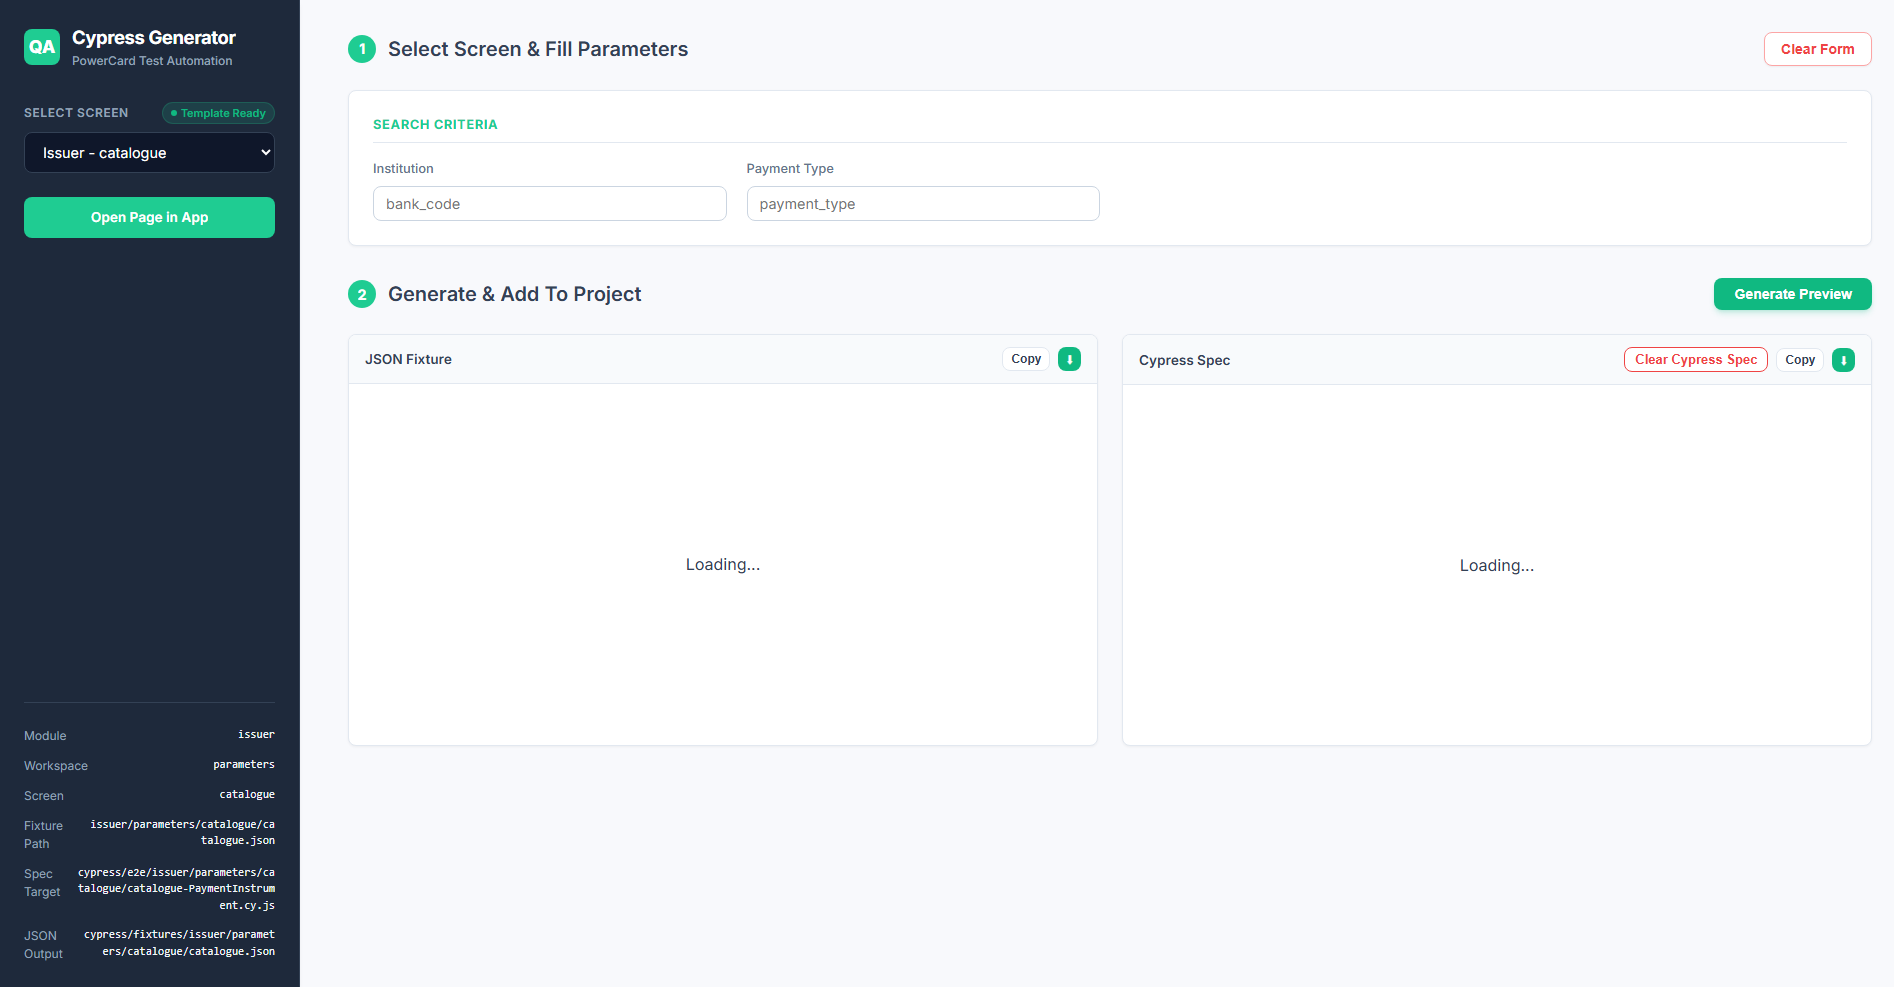
\includegraphics[width=\textwidth]{screenshots/chap-01.png}
\caption{Page d'accueil du Dashboard --- Vue globale de l'interface}
\end{figure}

L'interface d'accueil du Dashboard présente le menu latéral gauche (\textit{sidebar}) qui liste les 32 écrans PowerCARD catalogués, organisés par module (Switch, Issuer, Online, Acquiring). La zone centrale affiche les formulaires dynamiques et les éditeurs de code. Le design adopte un thème sombre professionnel avec des accents colorés pour la navigation.

\subsection{Étape 2 --- Sélection de l'écran MOTO}

\begin{figure}[H]
\centering
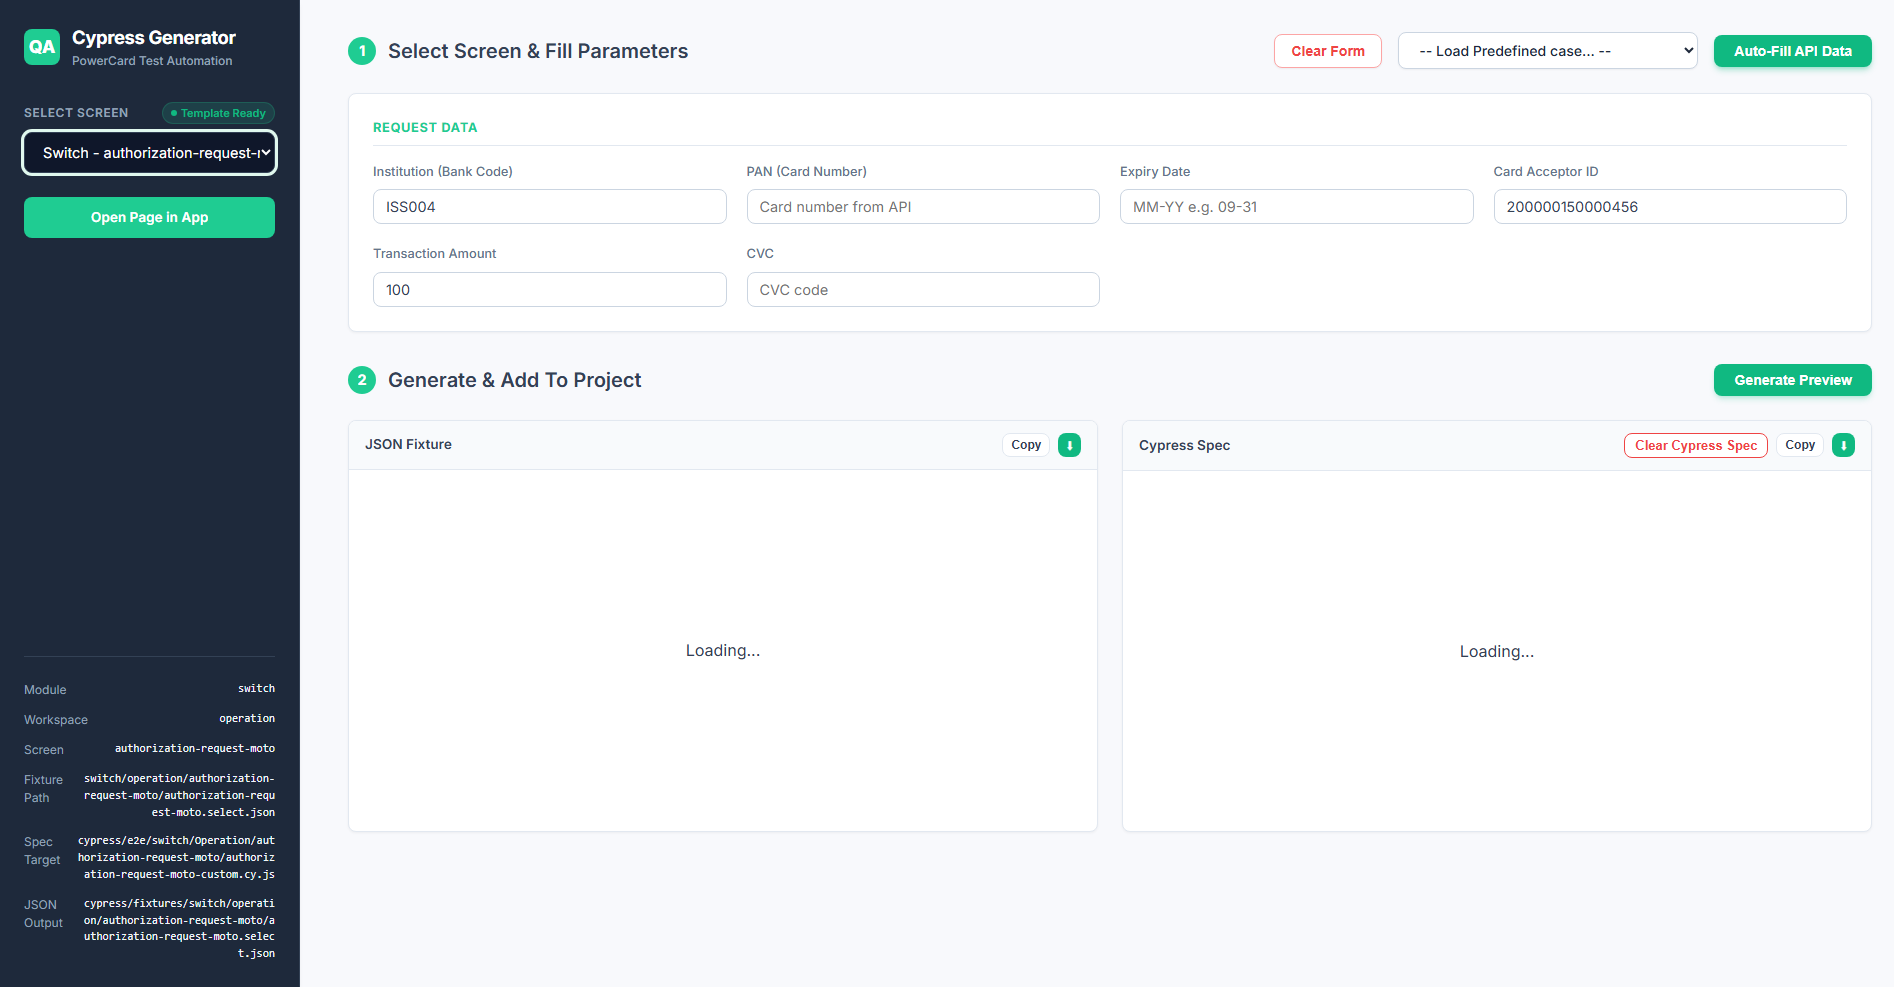
\includegraphics[width=\textwidth]{screenshots/chap-06.png}
\caption{Sélection de l'écran MOTO --- Le formulaire dynamique s'affiche automatiquement}
\end{figure}

En cliquant sur l'écran « Authorization Request MOTO » dans la sidebar, le Dashboard charge automatiquement le template de formulaire correspondant. Les champs affichés (Card Number, Expiry Date, Amount, Currency, etc.) sont spécifiques à ce type de transaction. Le système détecte le module (\texttt{switch}), le workspace (\texttt{operation}), et le chemin du spec Cypress associé.

\subsection{Étape 3 --- Auto-Fill API Data}

\begin{figure}[H]
\centering
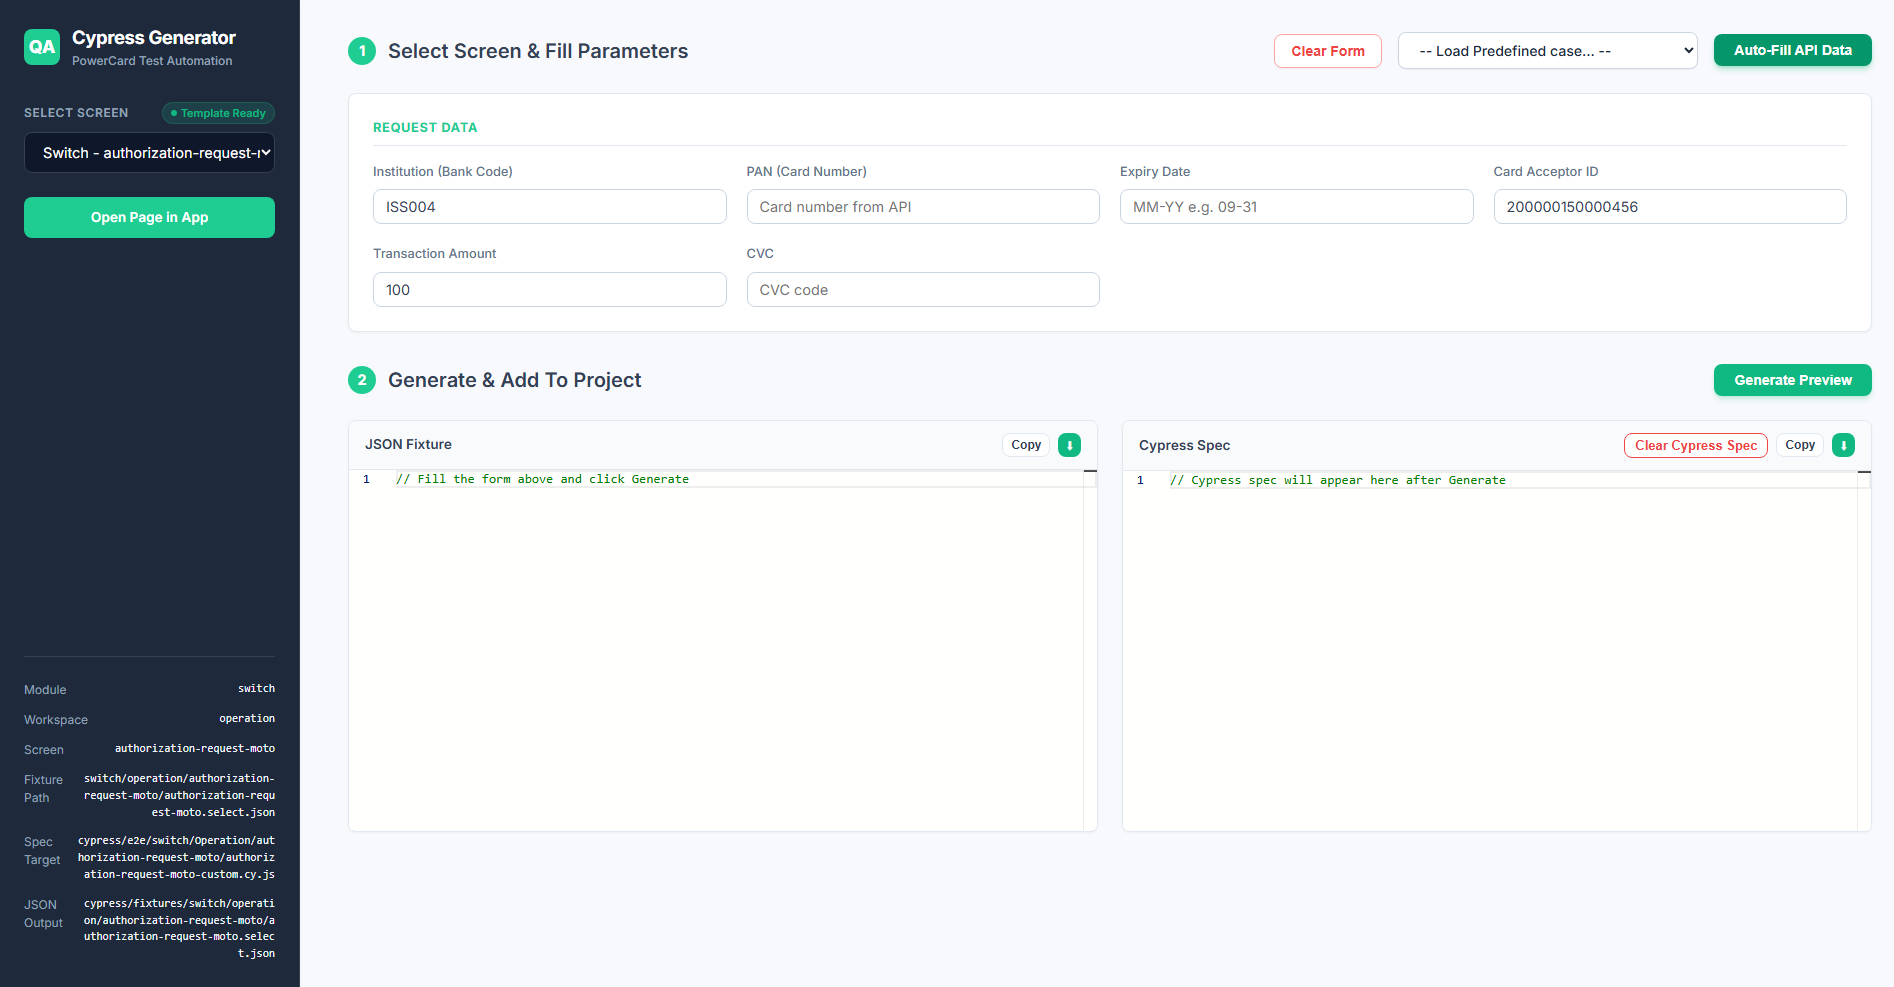
\includegraphics[width=\textwidth]{screenshots/chap-07.png}
\caption{Auto-Fill API Data --- Les données de carte sont récupérées automatiquement depuis l'API Connect}
\end{figure}

Le bouton « Auto-Fill API » déclenche un appel au proxy serveur qui s'authentifie auprès de l'API PowerCard Connect via JWT. Le système récupère automatiquement un numéro de carte de test valide, sa date d'expiration, et le code client associé. Ces données sont injectées dans les champs du formulaire, éliminant le besoin de saisie manuelle et garantissant la validité des données de test.

\subsection{Étape 4 --- Chargement d'un cas prédéfini}

\begin{figure}[H]
\centering
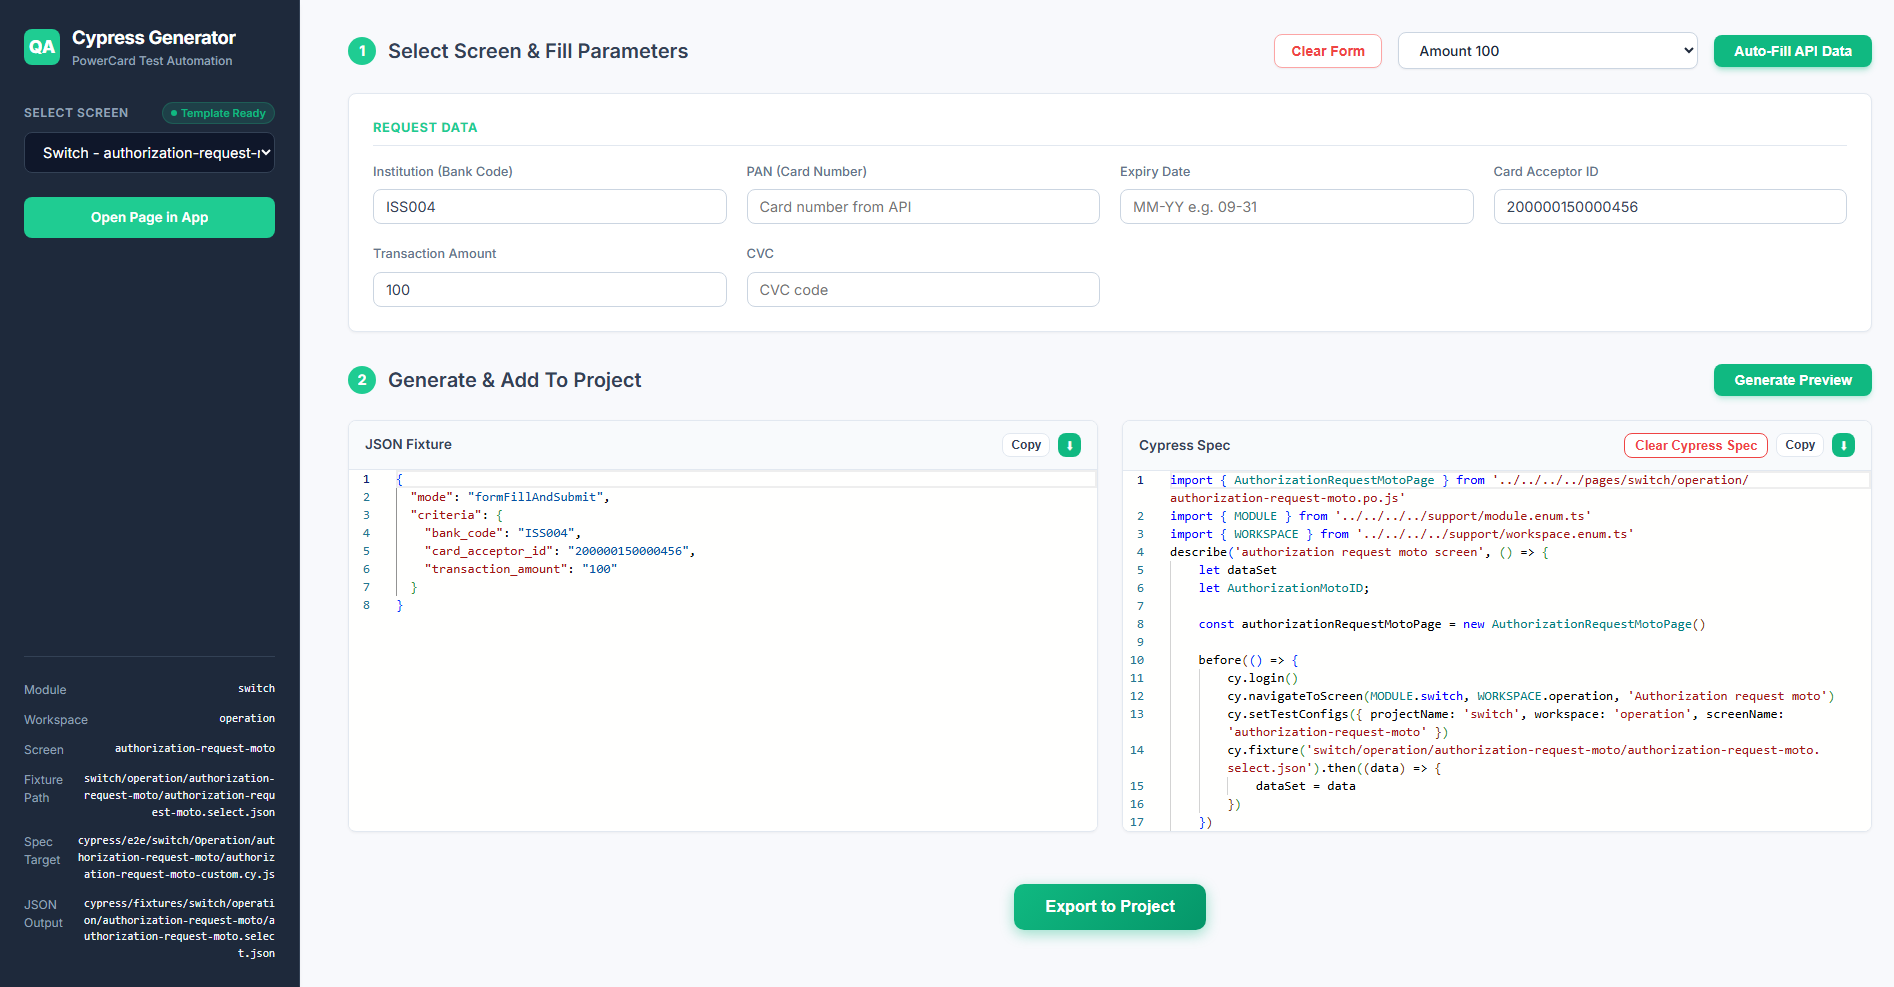
\includegraphics[width=\textwidth]{screenshots/chap-08.png}
\caption{Chargement d'un cas prédéfini --- Le montant de 100 est appliqué automatiquement}
\end{figure}

Le menu déroulant « Predefined Cases » permet de charger des jeux de données pré-configurés. Dans cet exemple, le cas « Amount 100 » remplit automatiquement le champ montant avec la valeur 100 et ajuste les autres paramètres de la transaction. Les cas prédéfinis sont définis dans \texttt{formTemplates.js} et permettent aux testeurs de reproduire rapidement des scénarios standards.

\subsection{Étape 5 --- Résultat de la génération}

\begin{figure}[H]
\centering
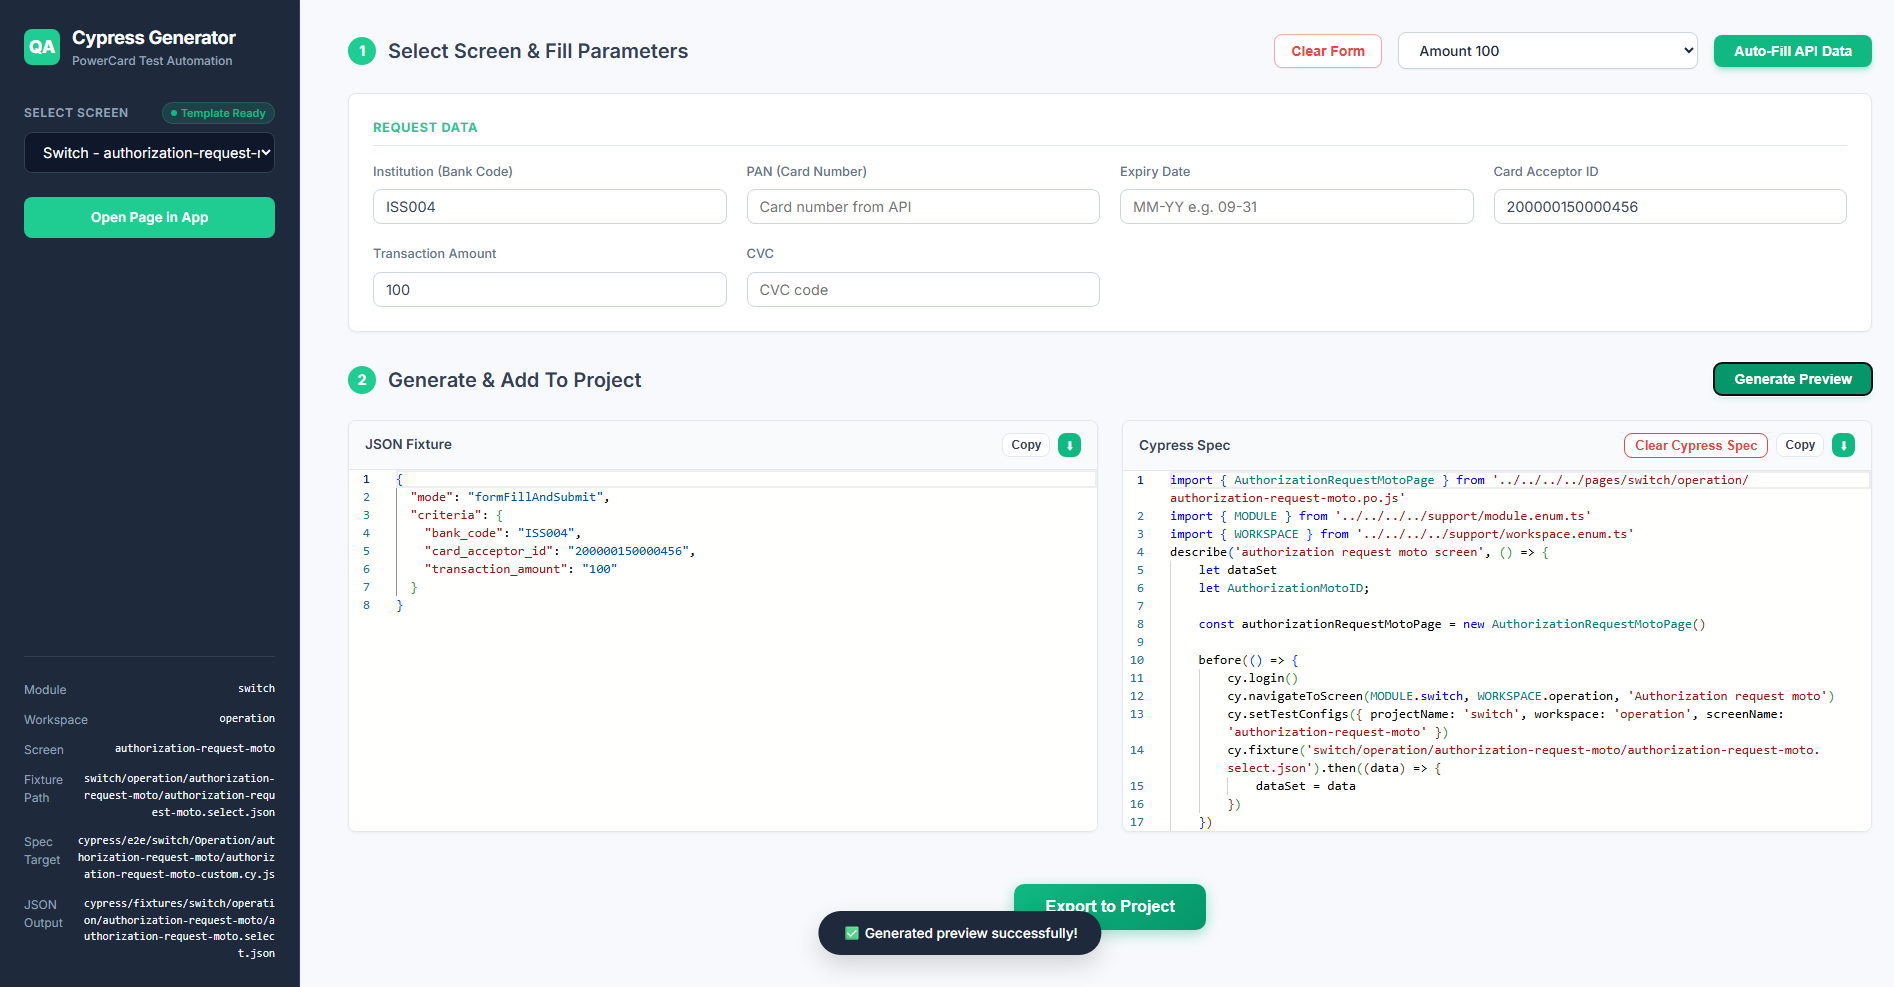
\includegraphics[width=\textwidth]{screenshots/chap-09.png}
\caption{Résultat de la génération --- Le JSON fixture et le Cypress Spec sont produits simultanément}
\end{figure}

Après avoir cliqué sur « Generate », le moteur de génération (\texttt{buildPayload()} + \texttt{patchSpec()}) produit simultanément deux fichiers : le \textbf{JSON fixture} contenant les données de test structurées, et le \textbf{Cypress Spec} (.cy.js) contenant le script de test complet. Les deux sont affichés côte à côte dans des éditeurs Monaco avec coloration syntaxique.

\subsection{Étape 6 --- Éditeurs Monaco}

\begin{figure}[H]
\centering
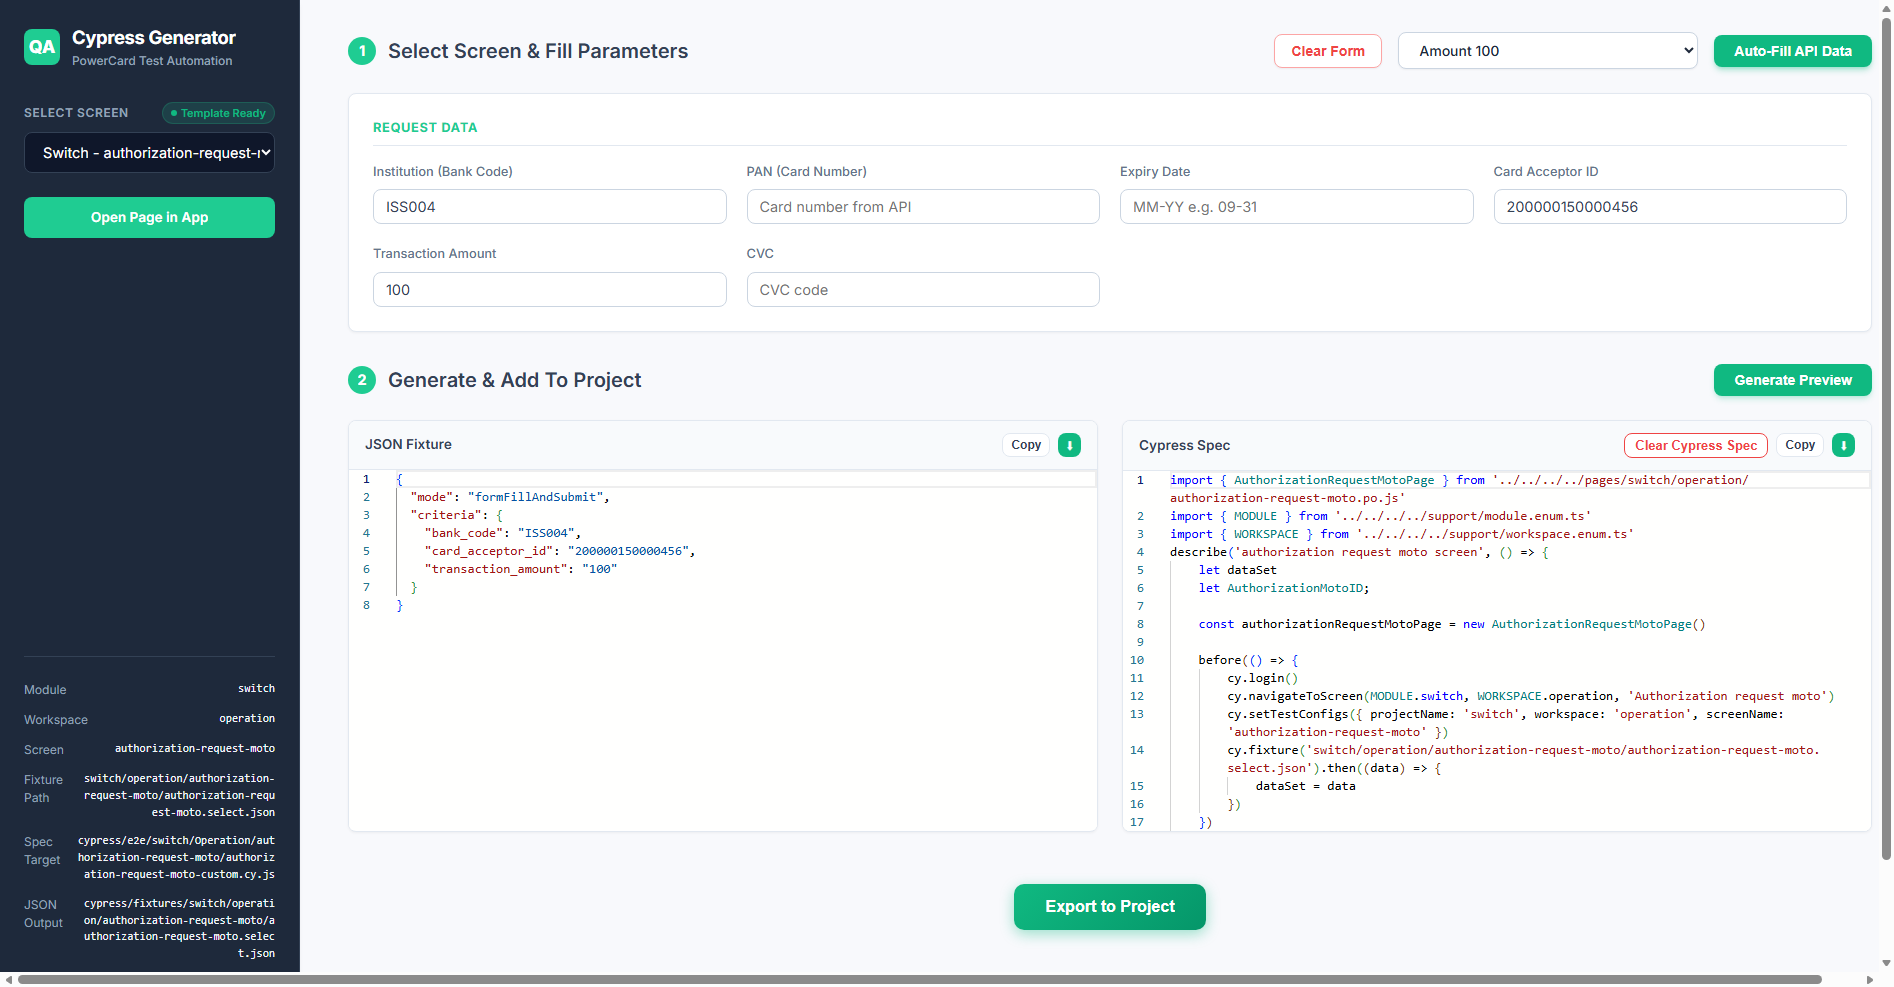
\includegraphics[width=\textwidth]{screenshots/chap-10.png}
\caption{Éditeurs Monaco --- Vue rapprochée avec coloration syntaxique JavaScript et JSON}
\end{figure}

Les éditeurs Monaco (le même moteur que VS Code) offrent une expérience de développement complète : coloration syntaxique, numérotation des lignes, pliage de code, et recherche. Le testeur peut vérifier et modifier le code généré avant de l'exporter. La partie gauche affiche le JSON fixture, la partie droite le script Cypress.

\subsection{Étape 7 --- Métadonnées dans la Sidebar}

\begin{figure}[H]
\centering
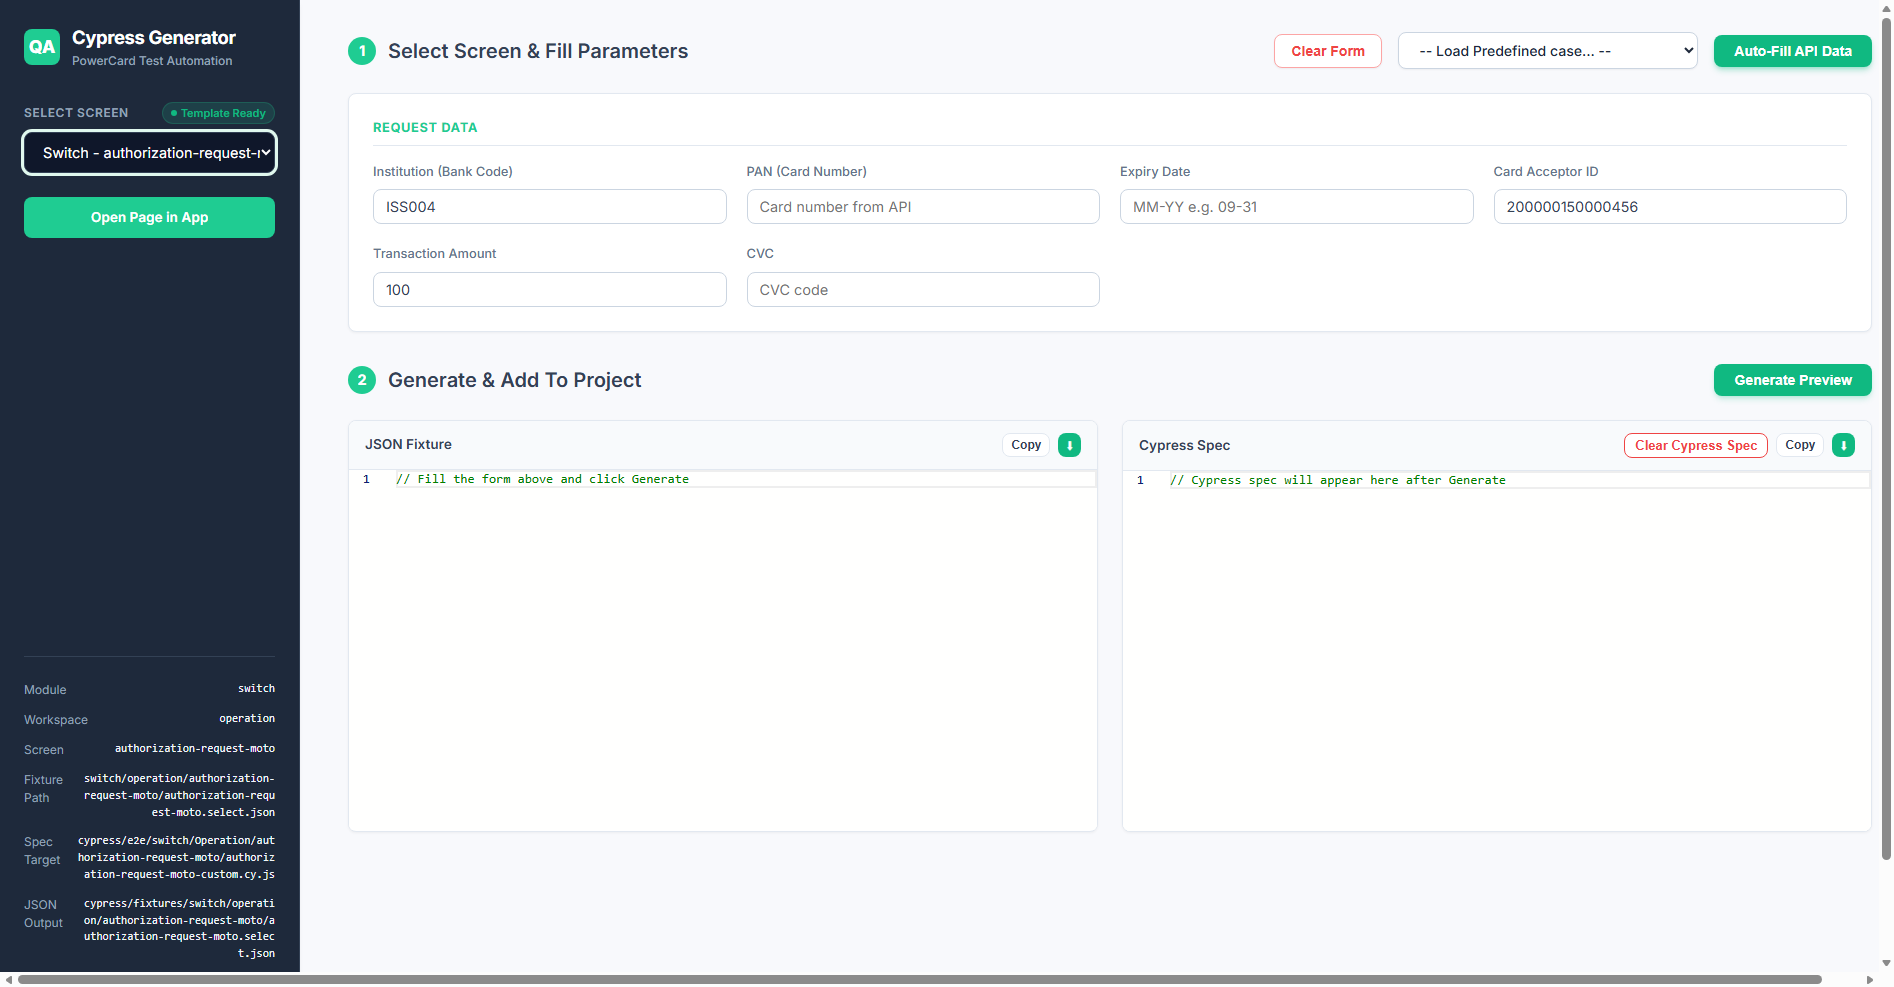
\includegraphics[width=\textwidth]{screenshots/chap-11.png}
\caption{Métadonnées de l'écran sélectionné --- Module, workspace, chemins des fichiers}
\end{figure}

La sidebar affiche les métadonnées complètes de l'écran sélectionné : le module (\texttt{switch}), le workspace (\texttt{operation}), le chemin du spec Cypress, le chemin du fixture JSON, et le nombre de champs du formulaire. Ces informations aident le testeur à comprendre l'organisation du projet et à localiser les fichiers générés.

\subsection{Étape 8 --- Module Issuer (autre exemple)}

\begin{figure}[H]
\centering
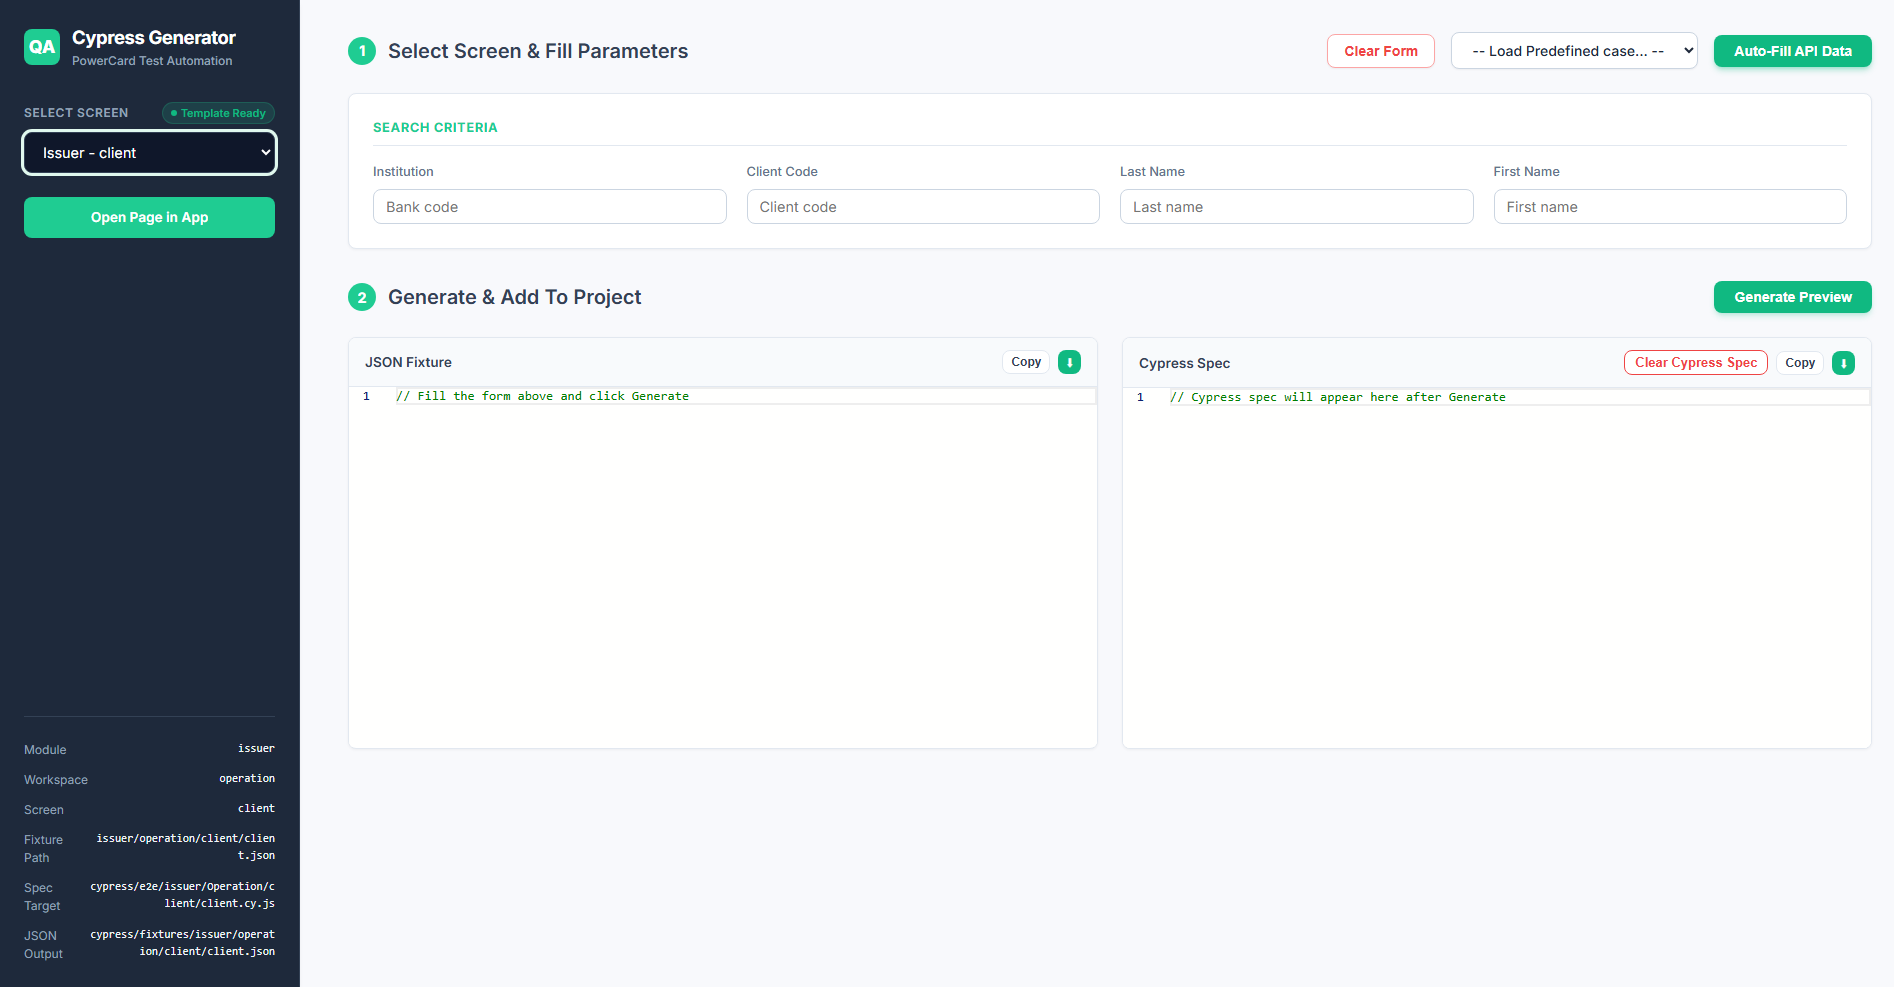
\includegraphics[width=\textwidth]{screenshots/chap-12.png}
\caption{Module Issuer --- L'écran Client avec ses champs spécifiques adaptés au contexte}
\end{figure}

Le Dashboard s'adapte dynamiquement au module sélectionné. Ici, l'écran « Client » du module Issuer affiche des champs différents de ceux du Switch MOTO : code institution, identifiant client, nom, adresse, etc. Cette flexibilité est rendue possible par le système de templates (\texttt{formTemplates.js}) qui mappe chaque écran à son formulaire spécifique.

\subsection{Étape 9 --- Export vers le projet}

\begin{figure}[H]
\centering
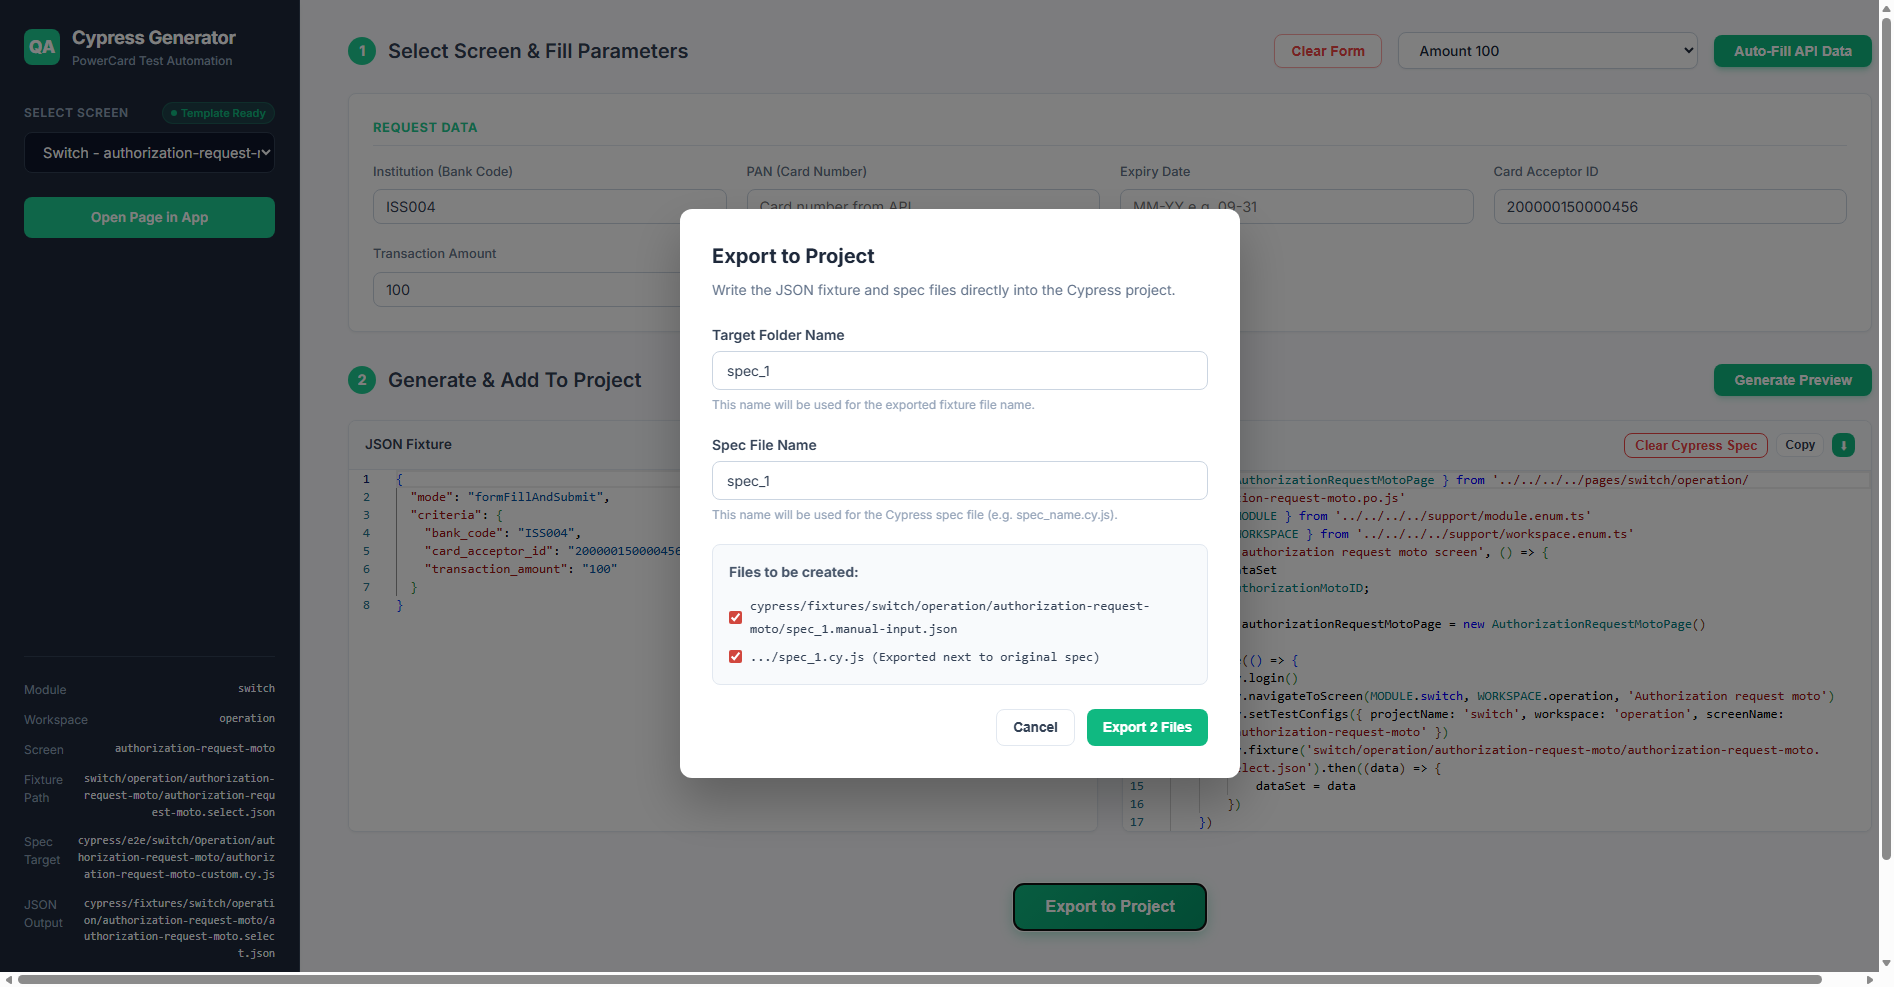
\includegraphics[width=\textwidth]{screenshots/chap-17-modal.png}
\caption{Modal d'export --- Confirmation avant écriture des fichiers dans l'arborescence Cypress}
\end{figure}

Le bouton « Export to Project » ouvre une modale de confirmation affichant les chemins exacts où les fichiers seront écrits : le fixture JSON dans \texttt{cypress/fixtures/} et le spec dans \texttt{cypress/e2e/}. Le serveur utilise \texttt{resolveSafeChildPath()} pour prévenir toute attaque de traversée de chemin avant d'écrire les fichiers via \texttt{fs.writeFileSync}.

\subsection{Étape 10 --- Exécution et rapport en temps réel}

\begin{figure}[H]
\centering
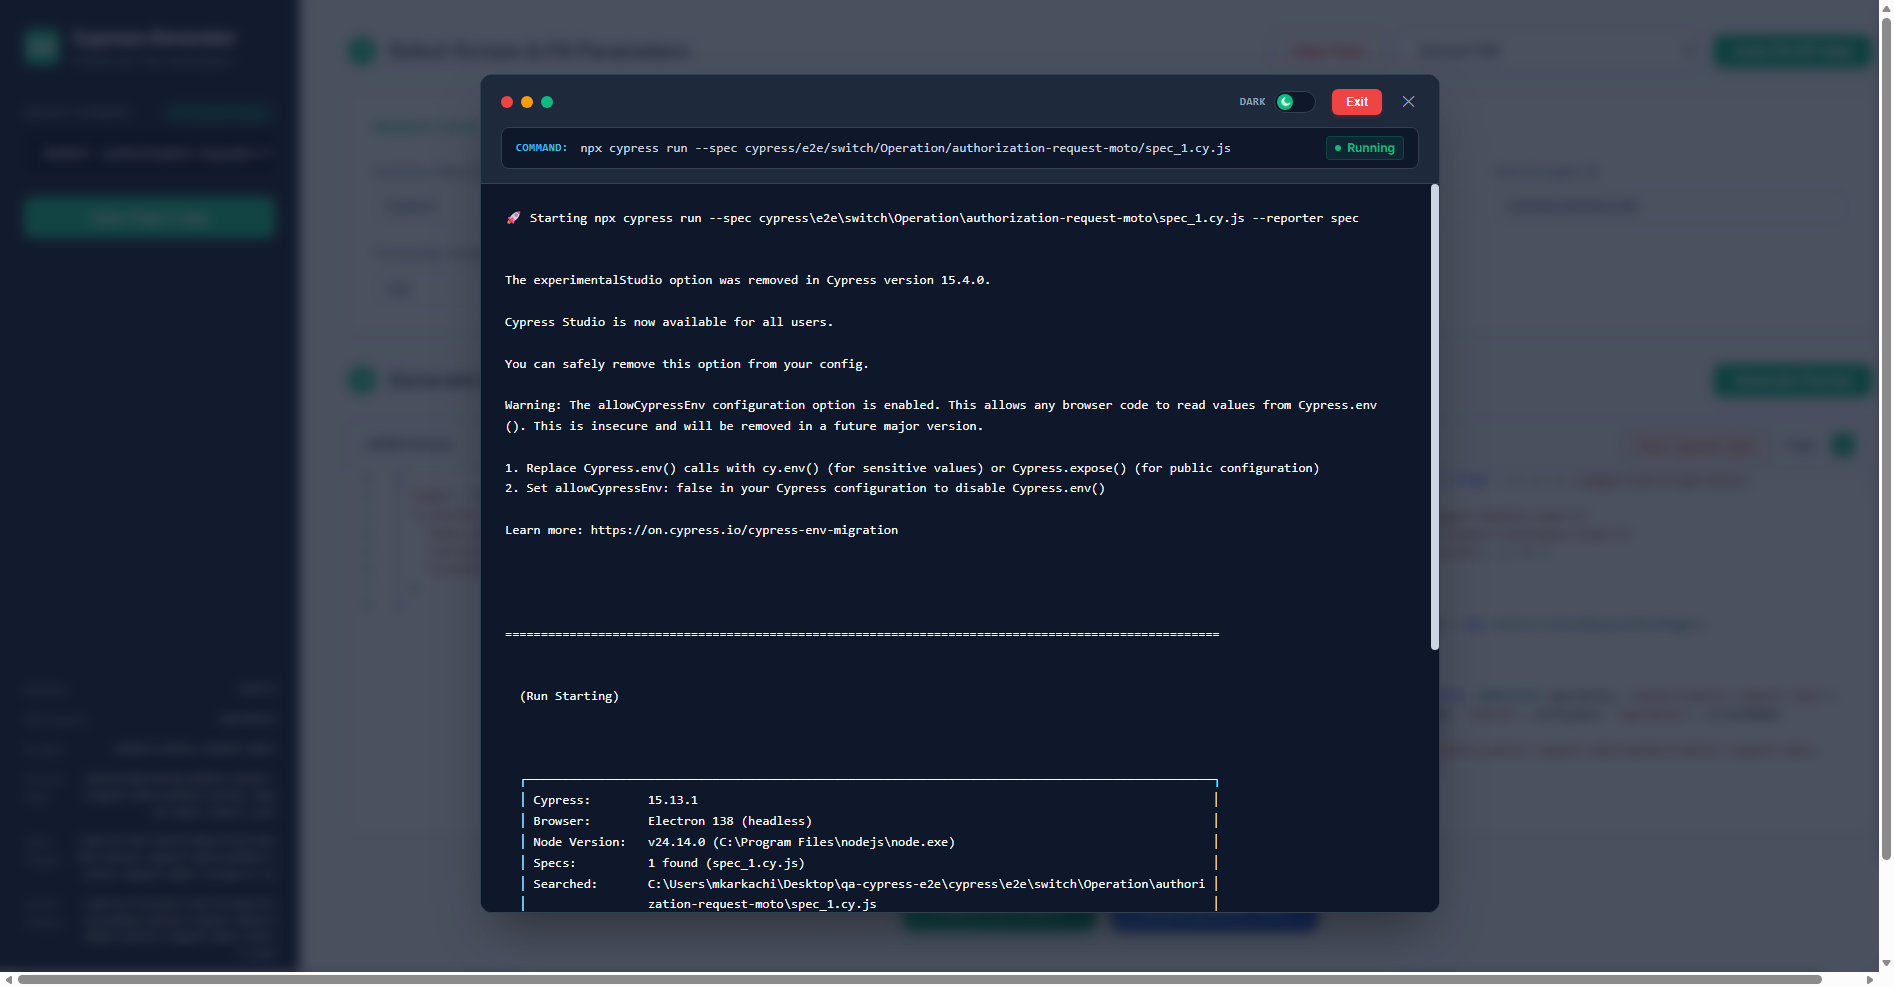
\includegraphics[width=\textwidth]{screenshots/chap-17-runner.png}
\caption{Terminal d'exécution intégré --- Les logs Cypress sont streamés en temps réel via SSE}
\end{figure}

Le terminal intégré dans le Dashboard affiche en temps réel les logs d'exécution du test Cypress. Le serveur Runner instancie un processus enfant (\texttt{spawn('npx cypress run --spec ...')}) et streame les sorties stdout/stderr via Server-Sent Events (SSE). Le parser \texttt{parseCypressLogs()} interprète les séquences d'échappement ANSI et colore les tests réussis en vert et les échecs en rouge.

\subsection{Étape 11 --- Résumé de l'exécution}

\begin{figure}[H]
\centering
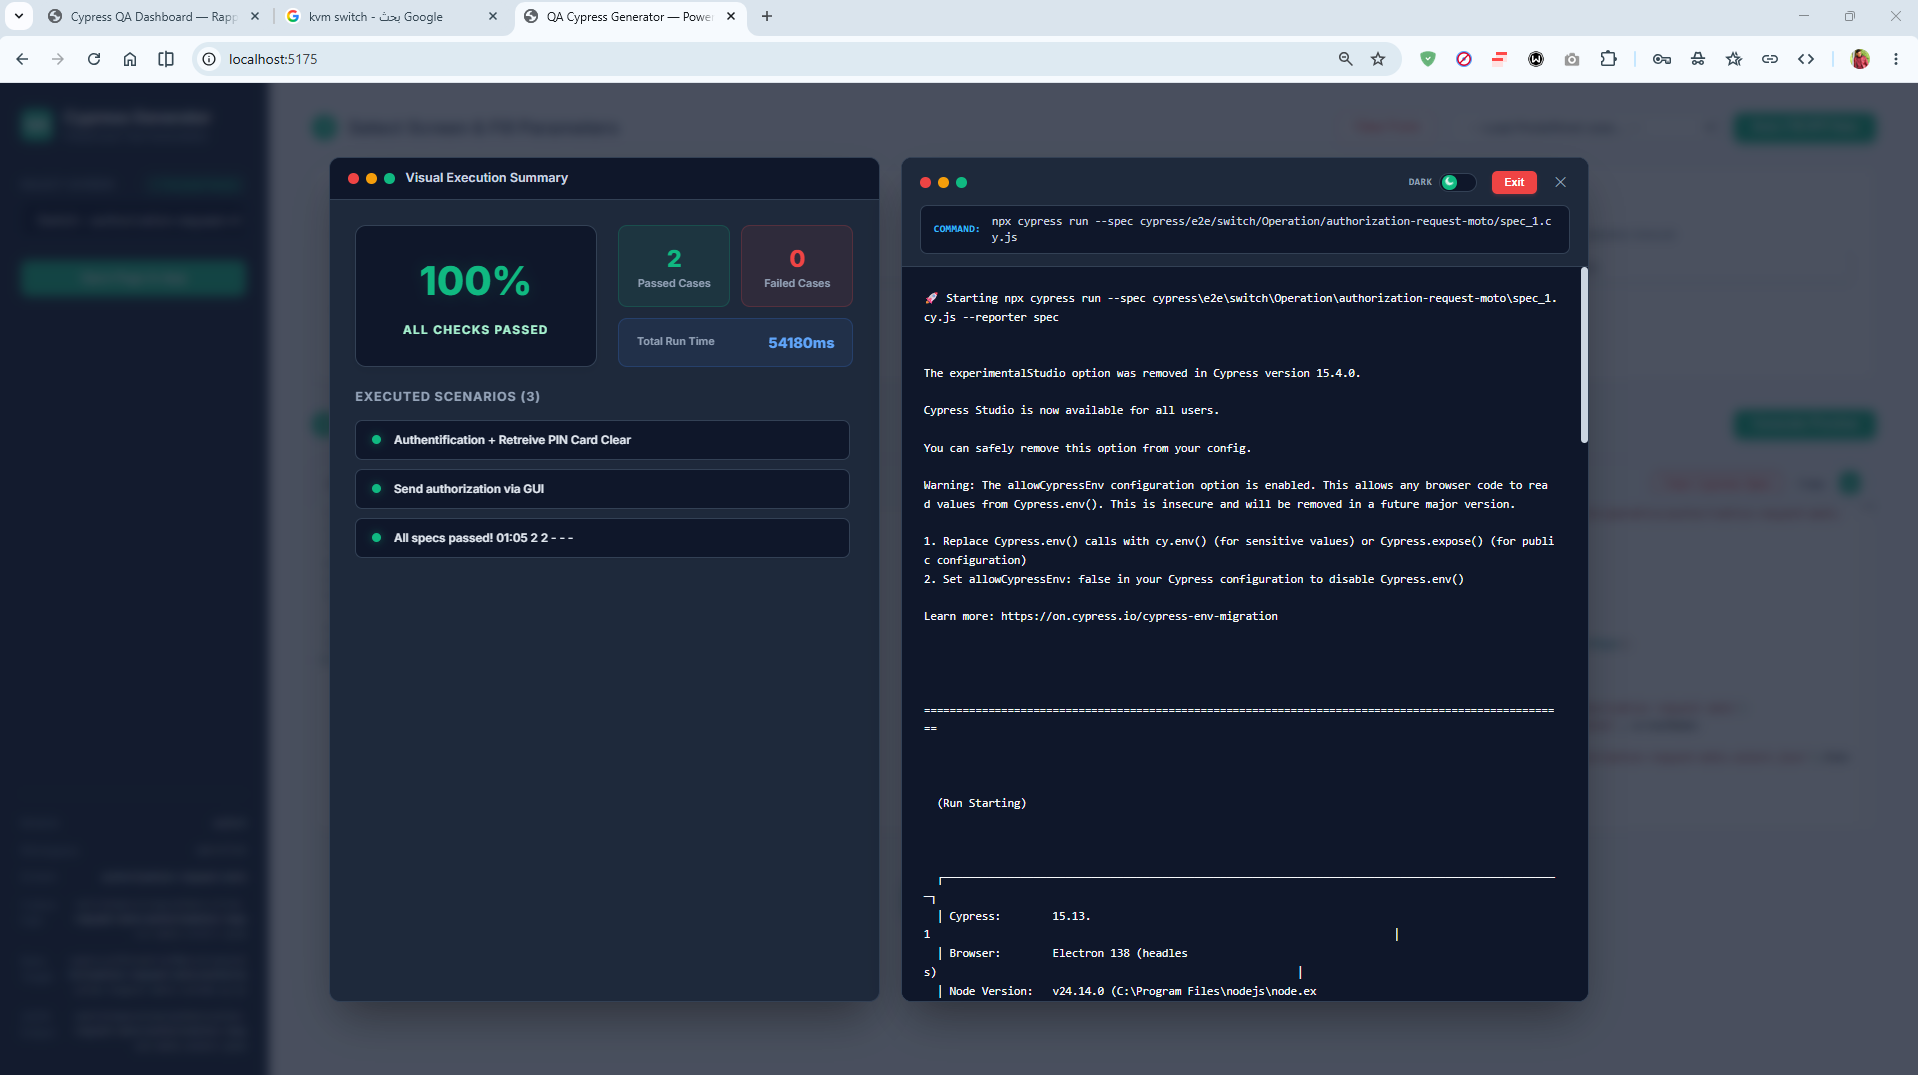
\includegraphics[width=\textwidth]{screenshots/chap-19-summary.png}
\caption{Résumé de l'exécution --- Pourcentage de succès, nombre de tests, et temps total}
\end{figure}

À la fin de l'exécution, le Dashboard affiche un résumé structuré : le pourcentage de réussite, le nombre de tests passés/échoués, et le temps total d'exécution. Cette vue synthétique permet aux testeurs de rapidement évaluer la qualité du module testé sans avoir à analyser les logs bruts.


% ══════════════════════════════════════════════════════════════════
% SECTION 3: RAPPORT QA --- CYCLE DE VIE DU TERMINAL
% ══════════════════════════════════════════════════════════════════
\newpage
\section{Rapport QA --- Cycle de vie du Terminal}

\textit{Cette section présente le rapport d'automatisation QA pour le scénario de test du Cycle de vie du Terminal, couvrant les fonctionnalités Network MCC Mapping et Merchant Onboarding sur PowerCARD V4.3.1-develop.}

\vspace{10pt}


\begin{tcolorbox}[colback=primary!5, colframe=primary, title=Aperçu du Projet \& Constats Critiques, arc=5pt]
    \begin{itemize}[leftmargin=1.5em]
        \item \textbf{Sujet :} Validation du Mapping Network MCC
        \item \textbf{Environnement :} Espaces de travail Administration \& Opération (V4.3.1-develop)
        \item \textbf{Statut d'exécution :} \textcolor{success}{8 Réussis}, \textcolor{warning}{0 Ignorés}, \textcolor{danger}{2 Échoués (Défauts)}
        \item \textbf{Date :} 2026-05-12
    \end{itemize}
    
    \vspace{0.3cm}
    \textbf{\large Résumé des bugs principaux (Journal Jira) :}
    \begin{itemize}[leftmargin=1.5em, itemsep=3pt]
        \item \textbf{BF-911 (Défaut) :} Les données ne sont pas conservées dans le champ obligatoire « Ville » après la confirmation de l'enregistrement.
        \item \textbf{BF-912 (Défaut) :} Interface - L'indicateur d'onglet dans la navigation latérale reste vert lorsqu'un champ obligatoire est en état d'erreur.
        \item \textbf{BF-916 (Défaut/Processus) :} [Network Mcc Mapping] Améliorations de la validation du tableau et du flux de travail.
        \item \textbf{BF-921 (Défaut Critique) :} [Network Mcc Mapping] L'enregistrement échoue avec une fenêtre d'erreur lorsque tous les champs sont remplis.
    \end{itemize}
\end{tcolorbox}

\subsection{Résumé de l'Exécution des Tests}

\begin{tcolorbox}[colback=primary!5, colframe=primary, title=\textbf{Résumé Exécutif}]
Ce cycle de test s'est concentré sur la fonctionnalité de \textbf{Mapping Network MCC du Marchand}. Sur 10 scénarios testés, 8 ont réussi, confirmant que la configuration de base et la navigation fonctionnent comme prévu. Cependant, un \textbf{problème bloquant critique} a été identifié lors de l'enregistrement d'une grille complète de mappings.
\end{tcolorbox}

\begin{center}
\renewcommand{\arraystretch}{1.5}
\begin{tabular}{|c|c|c|c|}
\hline
\textbf{Total CT} & \cellcolor{successbg}\textcolor{white}{\textbf{Réussis}} & \cellcolor{warningbg}\textcolor{white}{\textbf{Ignorés}} & \cellcolor{dangerbg}\textcolor{white}{\textbf{Échoués}} \\
\hline
\textbf{10} & \textcolor{successbg}{\textbf{8}} & \textcolor{warningbg}{\textbf{0}} & \textcolor{dangerbg}{\textbf{2}} \\
\hline
\end{tabular}
\end{center}

\subsection{Mapping Network MCC (\texttt{network-mcc-mapping.cy.js})}

\vspace{0.3cm}
\noindent
\begin{minipage}{\textwidth}
\renewcommand{\arraystretch}{1.5}
\begin{tabular}{|p{3cm}|p{12.5cm}|}
\hline
\rowcolor{primary}
\textcolor{white}{\textbf{Section}} & \textcolor{white}{\textbf{Détails}} \\
\hline
\multicolumn{2}{|c|}{\cellcolor{gray!20}\textbf{OPÉRATION DE LECTURE}} \\
\hline
\textbf{Bloc it()} & \texttt{it('READ: Verify screen and search MCC')} \\
\hline
\textbf{Actions} & $\bullet$ Vérifier les éléments de l'écran (champs MCC, bouton Ajouter).\newline $\bullet$ Rechercher en utilisant le code MCC 3847. \\
\hline
\textbf{Statut} & \textcolor{success}{\textbf{RÉUSSI}} \\
\hline
\end{tabular}
\end{minipage}

\vspace{0.5cm}
\noindent
\begin{minipage}{\textwidth}
\renewcommand{\arraystretch}{1.5}
\begin{tabular}{|p{3cm}|p{12.5cm}|}
\hline
\rowcolor{primary}
\textcolor{white}{\textbf{Section}} & \textcolor{white}{\textbf{Détails}} \\
\hline
\multicolumn{2}{|c|}{\cellcolor{gray!20}\textbf{OPÉRATION DE CRÉATION}} \\
\hline
\textbf{Bloc it()} & \texttt{it('CREATE: Add all networks, save and verify success')} \\
\hline
\textbf{Actions} & $\bullet$ Ajouter la première ligne (UPI) avec le MCC 7011.\newline $\bullet$ Ajouter récursivement tous les réseaux restants.\newline $\bullet$ Cliquer sur le bouton Enregistrer. \\
\hline
\textbf{Statut} & \textcolor{danger}{\textbf{ÉCHOUÉ}} (Défaut Critique \textbf{BF-921} - 500 Erreur interne) \\
\hline
\end{tabular}
\end{minipage}

\vspace{0.5cm}
\noindent
\begin{minipage}{\textwidth}
\renewcommand{\arraystretch}{1.5}
\begin{tabular}{|p{3cm}|p{12.5cm}|}
\hline
\rowcolor{primary}
\textcolor{white}{\textbf{Section}} & \textcolor{white}{\textbf{Détails}} \\
\hline
\multicolumn{2}{|c|}{\cellcolor{gray!20}\textbf{OPÉRATION DE MISE À JOUR}} \\
\hline
\textbf{Bloc it()} & \texttt{it('UPDATE: Modify MCC value, save and verify success')} \\
\hline
\textbf{Actions} & $\bullet$ Mettre à jour le code MCC de la première ligne (8888).\newline $\bullet$ Cliquer sur Enregistrer. \\
\hline
\textbf{Statut} & \textcolor{success}{\textbf{RÉUSSI}} \\
\hline
\end{tabular}
\end{minipage}

\vspace{0.5cm}
\noindent
\begin{minipage}{\textwidth}
\renewcommand{\arraystretch}{1.5}
\begin{tabular}{|p{3cm}|p{12.5cm}|}
\hline
\rowcolor{primary}
\textcolor{white}{\textbf{Section}} & \textcolor{white}{\textbf{Détails}} \\
\hline
\multicolumn{2}{|c|}{\cellcolor{gray!20}\textbf{OPÉRATION DE SUPPRESSION}} \\
\hline
\textbf{Bloc it()} & \texttt{it('DELETE: Remove a single row and verify')} \\
\hline
\textbf{Actions} & $\bullet$ Cliquer sur supprimer sur une ligne spécifique et confirmer. \\
\hline
\textbf{Statut} & \textcolor{success}{\textbf{RÉUSSI}} \\
\hline
\end{tabular}
\end{minipage}


\subsection{Merchant Onboarding (\texttt{merchant-onboarding.cy.js})}

\vspace{0.3cm}
\noindent
\begin{minipage}{\textwidth}
\renewcommand{\arraystretch}{1.5}
\begin{tabular}{|p{3cm}|p{12.5cm}|}
\hline
\rowcolor{primary}
\textcolor{white}{\textbf{Section}} & \textcolor{white}{\textbf{Détails}} \\
\hline
\multicolumn{2}{|c|}{\cellcolor{gray!20}\textbf{CRÉATION DU MARCHAND}} \\
\hline
\textbf{Bloc it()} & \texttt{it('CREATE: Fill all tabs and save Merchant')} \\
\hline
\textbf{Actions} & $\bullet$ Cliquer sur Nouveau.\newline $\bullet$ Remplir les onglets Description, Statut, Localisation.\newline $\bullet$ Cliquer sur Enregistrer. \\
\hline
\textbf{Statut} & \textcolor{success}{\textbf{RÉUSSI}} \\
\hline
\end{tabular}
\end{minipage}

\vspace{0.5cm}
\noindent
\begin{minipage}{\textwidth}
\renewcommand{\arraystretch}{1.5}
\begin{tabular}{|p{3cm}|p{12.5cm}|}
\hline
\rowcolor{primary}
\textcolor{white}{\textbf{Section}} & \textcolor{white}{\textbf{Détails}} \\
\hline
\multicolumn{2}{|c|}{\cellcolor{gray!20}\textbf{VÉRIFICATION PERSISTANCE}} \\
\hline
\textbf{Bloc it()} & \texttt{it('UPDATE: Open merchant, check City field')} \\
\hline
\textbf{Actions} & $\bullet$ Double-cliquer pour ouvrir les détails.\newline $\bullet$ Naviguer vers l'onglet Localisation.\newline $\bullet$ Vérifier si la valeur du champ Ville est conservée. \\
\hline
\textbf{Statut} & \textcolor{danger}{\textbf{ÉCHOUÉ}} (\textbf{BF-911} - Données non conservées dans le champ Ville) \\
\hline
\end{tabular}
\end{minipage}


% ── Étapes de Test avec Captures ──
\newpage
\subsection{Étapes de Test --- Captures d'écran}

\subsubsection{Connexion à PowerCARD}

\twoimages{login_empty.png}{Connexion PowerCARD --- Formulaire vide}
          {login_filled.png}{Connexion PowerCARD --- Identifiants remplis (ISS007)}

\begin{lstlisting}[caption={Code de connexion}]
cy.clearCookies()
cy.clearLocalStorage()
cy.login('ISS007', '*********')
cy.waitBusy()
\end{lstlisting}

\subsubsection{Navigation vers le Mapping Network MCC}

\twoimages{search_mcc.png}{Rechercher ``Network MCC mapping''}
          {empty_mcc.png}{Mapping Network MCC --- Formulaire vide}

\subsubsection{Saisie du Code MCC et Tests Négatifs}

\twoimages{loaded_mcc.png}{MCC 3847 chargé avec les données d'institution}
          {tc8.png}{Validation : Erreur de clé étrangère (test négatif)}

\subsubsection{Ajout des Mappings et Enregistrement}

\begin{figure}[H]
    \centering
    
\includegraphics[width=0.8\textwidth]{save_success.png}
    \caption{Opération enregistrée avec succès}
\end{figure}

\subsubsection{Intégration du Marchand (Espace Opération)}

\twoimages{op_dashboard.png}{Tableau de bord Opération}
          {pos_module.png}{Barre latérale du module Pos}

\twoimages{step12_empty.png}{Formulaire de marchand vide}
          {step13_desc.png}{Onglet Description rempli}

\twoimages{step14_loc.png}{Onglet Localisation}
          {step15_success.png}{Opération enregistrée avec succès}

\subsubsection{Vérification Finale}

\begin{figure}[H]
    \centering
    
\includegraphics[width=0.8\textwidth]{step16_result.png}
    \caption{Résultat final de la recherche --- Le marchand est trouvé dans la liste}
\end{figure}


% ── Journal des Tickets Jira ──
\newpage
\subsection{Journal Officiel des Tickets Jira}

\subsubsection{[BF-911] Données non conservées dans le champ Ville}

\begin{tcolorbox}[colback=white, colframe=primary, title=\textbf{Ticket Jira : BF-911}, fonttitle=\bfseries]
\textbf{Environnement :} \texttt{bo\_fe\_develop} | \textbf{Cluster :} \texttt{Andromed}

\textbf{Étapes :}
\begin{enumerate}[leftmargin=1.5em]
    \item Écran d'intégration du marchand → Nouveau → Remplir tous les champs → Enregistrer.
    \item Retour → Rechercher l'enregistrement → Double-cliquer → Aller à Localisation.
\end{enumerate}

\bugtable{Le champ \textbf{Ville} ne doit pas être vide.}
         {Le champ \textbf{Ville} est vide.}
\end{tcolorbox}

\subsubsection{[BF-912] Indicateur d'onglet incorrect}

\begin{tcolorbox}[colback=white, colframe=primary, title=\textbf{Ticket Jira : BF-912}, fonttitle=\bfseries]
\textbf{Environnement :} \texttt{bo-fe-develop} | \textbf{Cluster :} \texttt{Andromed}

\bugtable{L'onglet doit devenir rouge si des champs obligatoires sont manquants.}
         {L'onglet reste vert.}
\end{tcolorbox}

\twoimages{user_img4.png}{Résultat Attendu (L'onglet devient ROUGE)}
          {user_img3.png}{Résultat Obtenu (L'onglet reste VERT)}

\subsubsection{[BF-921] Enregistrement échoue --- Erreur critique}

\begin{tcolorbox}[colback=white, colframe=primary, title=\textbf{Ticket Jira : BF-921}, fonttitle=\bfseries]
\textbf{Environnement :} \texttt{bo-fe-develop} | \textbf{Cluster :} \texttt{Andromed}

\bugtable{Le mapping doit être enregistré avec succès.}
         {Erreur 500 : « Create Problem. Objects creation could not be performed ».}
\end{tcolorbox}

\begin{figure}[H]
    \centering
    
\includegraphics[width=0.8\textwidth]{failure.png}
    \caption{Preuve : Fenêtre d'erreur rouge lors de l'enregistrement}
\end{figure}


% ── Résumé des Bugs ──
\subsection{Résumé des Bugs}

\begin{center}
\renewcommand{\arraystretch}{1.4}
\begin{tabularx}{\textwidth}{|c|c|c|R|R|}
\hline
\rowcolor{primary!15}\textbf{\#} & \textbf{Type} & \textbf{Clé Jira} & \textbf{Titre} & \textbf{Description} \\
\hline
1 & \textcolor{danger}{\textbf{Défaut}} & BF-911 & Données non conservées dans le champ ``Ville'' & Le champ ville s'affiche vide après confirmation et réouverture. \\
\hline
2 & \textcolor{danger}{\textbf{Défaut}} & BF-912 & L'indicateur d'onglet reste vert & L'onglet reste VERT même avec des champs obligatoires en erreur. \\
\hline
3 & \textcolor{warning}{\textbf{Défaut/Processus}} & BF-916 & Validation du tableau & Lignes infinies, validation longueur manquante, infobulles absentes. \\
\hline
4 & \textcolor{danger}{\textbf{Défaut Critique}} & BF-921 & Enregistrement échoue & Erreur 500 lors de l'enregistrement de l'ensemble des mappings. \\
\hline
\end{tabularx}
\end{center}


\vspace{10pt}
\textbf{Conclusion}

En conclusion, ce chapitre a concrétisé l'aboutissement de mon projet de fin d'études en démontrant la viabilité technique des solutions proposées. L'automatisation réussie des flux fonctionnels PowerCARD garantit une détection rapide et fiable des régressions. La démonstration pratique du flux MOTO a illustré de manière concrète comment le Dashboard permet à un testeur de générer, exporter et exécuter un test complet en quelques minutes, sans écrire une seule ligne de code. Parallèlement, le rapport QA a mis en évidence la capacité de l'outil à identifier des défauts critiques dans l'application. Le dernier chapitre s'attachera à évaluer le bilan de ce projet et ses apports globaux.
